\chapter{Aspectos Teóricos}
\noindent
En este capítulo se presentan los prerrequisitos necesarios para obtener los resultados que se
encuentran a lo largo de esta tesis. En primer lugar, en la sección \ref{sec:prerreq} se recopilan
resultados básicos de teoría de números y de programación lineal que forman parte de la literatura
tradicional y constituyen nuestras bases a partir de las cuales derivaremos nuestros propios
resultados. En segundo lugar, en la sección \ref{sec:foundations} se presentan enunciados y definiciones
obtenidos de \cite{herr}, los cuales utilizaremos para continuar con la construcción de nuestros
resultados originales.

Como mencionamos en la introducción de esta tesis, nos concentraremos casi exclusivamente en problemas
de programación lineal entera del tipo
\begin{subequations}
	\label{theory:formulation}
	\begin{align}
		\max_{\vec{x} \in \Z^n} \quad
			& \vec{p}^T\vec{x}, \label{theory:objective} \\
		\text{s.a.} \quad
			& \vec{p}^T\vec{x} \leq u, \label{theory:constraint:budget} \\
			& \vec{x} \geq \vec{0}, \nonumber
	\end{align}
\end{subequations}
donde $\vec{p}\in\R\setminus\braces{\vec{0}}$ pertenece a una clase que definiremos en la sección
\ref{sec:foundations} y $u \in \R$ es un escalar. Comúnmente haremos referencia a la restricción
\eqref{theory:constraint:budget} como \textbf{restricción presupuestaria} debido a que cada unidad
de $x_i$ ``cuesta'' $p_i$ unidades y queremos maximizar nuestro ``gasto''
\eqref{theory:objective} sin exceder nuestro \textbf{presupuesto} $u$. Podemos suponer, sin pérdida
de generalidad, que todas las entradas de $\vec{p}$ son distintas de cero. En efecto, si alguna
entrada $p_i$ es nula, cualquier elección entera y no negativa de $x_i$ es válida para este programa
lineal entero. Esta suposición será implícita en lo que resta del capítulo, aunque se hará explícita
al final cuando investiguemos la manera de clasificar instancias de este programa lineal entero.

\section{Prerrequisitos}
\label{sec:prerreq}
\noindent
Se consideró pertinente no incluir demostraciones en esta sección, pues los enunciados son
mostrados en los cursos de álgebra superior, programación lineal, o investigación de
operaciones. Las referencias principales para las subsecciones de teoría de números y de
programación lineal son \cite{carmen} y \cite{fabs}, respectivamente.

\subsection{Teoría de Números}
\label{section:number-theory}
\subsubsection{Máximo común divisor y mínimo común múltiplo}
\noindent

\begin{definition}
	Dados dos enteros $a$ y $b$, decimos que \textbf{$a$ divide a $b$} (y escribimos $a \mid b$) si
	existe un entero $k$ tal que $a = k \cdot b$. También denotamos por $D(a)$ al \textbf{conjunto de
	divisores de $a$}, es decir, definimos
	\begin{equation*}
		D(a) \coloneq \braces{b \in \Z \vcentcolon b \mid a}.
	\end{equation*}
\end{definition}
Observemos que si $a$ es distinto de cero, entonces $D(a)$ es finito. En efecto, si $b \mid a$ y $a
\neq 0$, es posible mostrar que $|b| \leq |a|$, lo cual implica que $|D(a)| \leq 2|a|$, donde
$|D(a)|$ denota la cardinalidad del conjunto $D(a)$ y $|a|$ el valor absoluto de $a$. En caso de que
$a$ sea nulo, se sigue que $D(a) = \Z$.
% \begin{observation}
% 	Para cualquier entero $a$ se satisface $\lbrace -1, 1 \rbrace \subseteq D(a)$, pues $a = a \cdot
% 	1$ y también $a = (-a) \cdot (-1)$.
% \end{observation}

\begin{definition}
	\label{prerreq:def:gcd}
	Sean $a_1, \ldots, a_n$ enteros no todos iguales a cero, entonces definimos su \textbf{máximo
	común divisor} $d$ como el máximo elemento del conjunto $\bigcap_{i=1}^{n}D(a_i)$, y escribimos
	$d = \gcd{a_1, \ldots, a_n}$. Si $d = 1$, entonces decimos que $a_1, \ldots, a_n$ son
	\textbf{coprimos}.
\end{definition}
Puesto que alguna entrada $a_i$ es distinta de cero en la definición anterior, encontramos que el
conjunto $\bigcap_{i=1}^{n}D(a_i)$ es finito y también es no vacío, por lo que este conjunto tiene
un máximo elemento. Es decir, el máximo común divisor está bien definido.

Además, el máximo común divisor siempre es positivo, pues se cumple que $1 \in D(a)$ para todo
entero $a$, lo que implica por maximalidad que $1 \leq \gcd{a_1, \ldots, a_n}$ para cualquier
colección de enteros no todos nulos.

La definición más común del máximo común es dada de manera inductiva. Decimos que $d$ es el máximo
común divisor de dos enteros $a_1, a_2$, no ambos iguales a cero, si se satisface
\begin{enumerate}
	\item $d \mid a_1$ y $d \mid a_2$, y también,
	\item si $d' \mid a_1$ y $d' \mid a_2$, entonces $d' \mid d$.
\end{enumerate}
Luego, para un conjunto de enteros $a_1, a_2 \ldots a_n$, no todos iguales a cero, definimos el máximo común
divisor entre ellos de manera inductiva:
\begin{equation*}
	\gcd{a_1, a_2, \ldots, a_{n-1}, a_n} \coloneq \gcd{a_1, \gcd{a_2, \ldots, \gcd{a_{n-1}, a_n} \cdots }}.
\end{equation*}
Sin embargo, debemos ser cuidadosos con esta manera de definir las cosas, pues puede ser el caso,
por ejemplo, que $a_{n-1}$ y $a_n$ sean ambos cero y entonces $\gcd{a_{n-1}, a_n}$ no está bien definido.

Para que esta manera de definir el máximo común divisor sea equivalente a la definición
\ref{prerreq:def:gcd}, deberemos presuponer o bien que $a_{n - 1} \neq 0$ o bien que $a_n \neq 0$. A
partir de este punto usaremos ambas definiciones de manera indistinta. Independientemente de la
definición que utilicemos, es posible calcular el máximo común divisor a través del algoritmo
de Euclides.

% \begin{observation}
% 	No porque una colección de enteros sea coprima se sigue que estos enteros son coprimos a pares.
% 	Por ejemplo, los enteros 1, 3 y 3 son coprimos pero evidentemente 3 y 3 no lo son.
% \end{observation}

\begin{definition}
	Decimos que $c \in \Z$ es una \textbf{combinación lineal entera} de un conjunto de enteros $a_1, \ldots,
	a_n$ si existen enteros $x_1, \ldots, x_n$ tales que $c = a_1x_1 + \cdots + a_nx_n$. Si $c$ es
	positivo, también decimos que esto último es una \textbf{combinación lineal entera positiva}.
\end{definition}
\begin{theorem}
	\label{prerreq:th:bezout}
	Sea $d$ un entero y sea $a_1, \ldots, a_n$ una colección de enteros no todos iguales a cero.
	Entonces $d = \gcd{a_1, \ldots, a_n}$ si y solo si $d$ es la mínima combinación lineal entera
	positiva de $a_1, \ldots, a_n$.
\end{theorem}
\begin{example}
	El máximo común divisor de los enteros 2, 3 y 5 es 1. Observemos que $-3\cdot 2 - 1\cdot 3 +
	2\cdot 5 = 1$.
\end{example}

\begin{lemma}
	\label{prerreq:lemma:gcd}
	Si $d = \gcd{a_1, \ldots, a_n}$, entonces $\gcd{\frac{a_1}{d}, \ldots, \frac{a_n}{d}} = 1$.
\end{lemma}

Además del máximo común divisor, haremos uso del mínimo común múltiplo, aunque será en menor medida.
\begin{definition}
	Definimos el \textbf{conjunto de múltiplos} de un entero $a$ como
	\begin{equation*}
		M(a) \coloneq \braces{x \in \Z \vcentcolon a \mid x}.
	\end{equation*}
	También definimos el \textbf{mínimo común múltiplo} de un conjunto de enteros $a_1, \ldots,
	a_n$, no todos iguales a cero, como el mínimo elemento del conjunto
	\begin{equation*}
		\Z_{\geq 0} \cap \bigcap_{i=1}^{n}M(a_i).
	\end{equation*}
	Escribimos $\lcm{a_1, \ldots, a_n}$ para denotar a este mínimo común múltiplo.
\end{definition}

% \begin{observation}
% 	Si $a$ es nulo, entonces $M(a) = \braces{0}$. En caso contrario encontramos que $M(a)$ es un
% 	conjunto infinito.
% \end{observation}

Para mostrar que el mínimo común múltiplo está bien definido, basta observar que el producto $|a_1
\cdots a_n|$ es no negativo y también es un elemento de $M(a_i)$ para toda $i \in \braces{1, \ldots,
n}$.

\subsubsection{Ecuaciones lineales diofantinas}

\noindent
Sea $c \in \Z$ y sea $a_1, \ldots, a_n$ una colección de enteros. Una ecuación
lineal diofantina es una ecuación en la que deseamos determinar enteros $x_1,
\ldots, x_n$ que satisfagan
\begin{equation*}
	a_1x_1 + \cdots + a_nx_n = c.
\end{equation*}
En esta sección nos enfocamos en el caso $n = 2$, y en la sección \ref{sec:foundations}
generalizamos estos resultados para cualquier entero $n \geq 2$. Los siguientes enunciados abordan
el problema de determinar la existencia y construcción de soluciones para este tipo de ecuaciones.
\begin{theorem}[Existencia]
	\label{prerreq:th:existence}
	Sean $a$ y $b$ enteros, no ambos iguales a cero. Entonces la ecuación lineal diofantina $ax + by
	= c$ tiene solución entera si y solo si $\gcd{a, b} \mid c$.
\end{theorem}
Para construir el conjunto de soluciones de una ecuación lineal diofantina, primero encontramos  una
solución particular.
\begin{definition}
	\label{prerreq:def:bezout}
	Sea $d \coloneq \gcd{a, b}$ y sean $x', y'$ números enteros tales que $ax' + by' = d$ (su
	existencia está garantizada por el teorema \ref{prerreq:th:bezout}). Decimos entonces que $x',
	y'$ son \textbf{coeficientes de Bézout} asociados a
	$a$ y $b$, respectivamente.
\end{definition}
Los coeficientes de Bézout se pueden calcular a través del algoritmo extendido
de Euclides. Observemos que estos coeficientes no son únicos. En efecto, si
$x', y'$ son coeficientes de Bézout de $a$ y $b$, entonces $x' + b$, $y' - a$
también lo son:
\begin{equation*}
	a(x' + b) + b(y' - a) = ax' + by' + ab - ab = ax' + by' = d.
\end{equation*}
Para fines de esta tesis basta la existencia de estos coeficientes, por lo que diremos de manera
indistinta ``los coeficientes de Bézout'' y ``una elección de coeficientes de Bézout''.

Definamos $d \coloneq \gcd{a, b}$ y supongamos que la ecuación $ax + by = c$ tiene solución.
Por el teorema \ref{prerreq:th:existence}, se sigue que $d \mid c$, y entonces existe $c' \in \Z$
tal que $c = c' \cdot d$. Sean $x', y'$ los coeficientes de Bézout asociados a $a, b$
respectivamente. Así,
\begin{equation*}
	a(c' \cdot x') + b(c' \cdot y') = c'(ax' + by') = c'd = c,
\end{equation*}
por lo que $(c' \cdot x', c' \cdot y')$ es una solución particular de la ecuación $ax + by = c$.

\begin{theorem}[Construcción]
	\label{prerreq:th:construction}
	Sea $ax + by = c$ una ecuación lineal diofantina con solución particular $(x_0, y_0)$, entonces
	todas sus soluciones están dadas por
	\begin{equation}
		\label{prerreq:eq:construction}
		\begin{cases}
			x = x_0 + \frac{b}{d}t, \\
			y = y_0 - \frac{a}{d}t,
		\end{cases}
	\end{equation}
	donde $d \coloneq \gcd{a, b}$ y $t \in \Z$ es una variable libre.
\end{theorem}

\begin{example}
	Consideremos la ecuación lineal $2x + 3y = 5$. Los coeficientes de Bézout asociados a 2 y 3 son,
	respectivamente, -1 y 1. Luego, una solución particular para la ecuación es $(x_0, y_0) = (-5, 5)$.
	Por el teorema anterior encontramos que todas las soluciones están dadas por
	\begin{equation*}
		\begin{cases}
			x = -5 + 3t, \\
			y = 5 - 2t,
		\end{cases}
	\end{equation*}
	donde $t \in \Z$ es una variable libre. En efecto, sustituyendo obtenemos
	\begin{equation*}
		2(-5 + 3t) + 3(5 - 2t) = -10 + 15 + 6t - 6t = 5.
	\end{equation*}
\end{example}

\subsection{Programación lineal}
\label{subsec:lp}
\noindent
\begin{definition}
	Sea $A \in \R^{m \times n}$ una matriz con renglones linealmente independientes y $\vec{b} \in
	\R^m$ un vector. Entonces al conjunto definido por
	\begin{equation}
		\label{prerreq:def:poly}
		P \coloneq \lbrace \vec{x} \in \R^n \colon A\vec{x} \geq \vec{b} \rbrace
	\end{equation}
	lo llamamos \textbf{poliedro}. Si, además, $P$ es acotado, entonces decimos que $P$ es un
	\textbf{politopo}.
\end{definition}

La programación lineal se encarga de resolver problemas de optimización de la forma
\begin{equation}
	\label{prim:lineal-opt}
	\max_{\vec{x} \in \R^n} ~\lbrace \vec{c}^T\vec{x} \colon \vec{x} \in P \rbrace,
\end{equation}
donde $P \subseteq \R^n$ es un poliedro al cual llamamos \textbf{región factible}, $\vec{c} \in \R^n$ un vector,
comúnmente conocido como el \textbf{vector objetivo}, y $\vec{x} \in \R^n$ un vector de variables a decidir.

% En esta sección repasamos brevemente algunas propiedades de la región factible $P$. Así también,
% indicamos dónde se encuentra el óptimo del problema \eqref{prim:lineal-opt} y hacemos mención rápida
% sobre cómo obtenerlo. Finalmente, nos enfocamos en programas lineales enteros y, más
% importantemente, describimos cómo funciona el algoritmo de Ramificación y Acotamiento para encontrar
% soluciones de estos programas enteros.

\begin{definition}
	Sea $\vec{a} \in \R^n$ un vector no nulo y sea $b \in \R$ un escalar. Llamamos
	\textbf{hiperplano afín}
	al conjunto de vectores $\vec{x} \in \R^n$ que satisfacen $\vec{a}^T\vec{x} = b$. Así también,
	llamamos \textbf{semi-espacios afines} a los conjuntos de vectores $\vec{x}, \vec{y} \in \R^n$ que
	satisfacen $\vec{a}^T\vec{x} \geq b$ y $\vec{a}^T\vec{y} \leq b$.
\end{definition}

Observemos que todo poliedro $P$ es la intersección de $m$ semi-espacios afines. Esto se debe a que,
para una matriz $A \in \R^{m \times n}$ con renglones independientes y un vector $\vec{b} \in \R^m$,
$A\vec{x} \geq \vec{b}$ si y solo si $\vec{a}_i^T\vec{x} \geq b_i$ para toda $1 \leq i \leq m$ y
donde $\vec{a}_i^T$ denota el $i$-ésimo renglón de la matriz $A$. En la figura \ref{fig:hyp} se
muestra la relación entre semi-espacios afines y poliedros.

\begin{figure}[ht]
	\centering
	\begin{minipage}{0.45\textwidth}
		\centering
		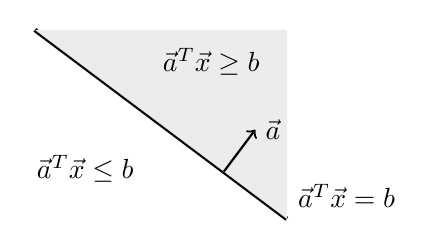
\begin{tikzpicture}[scale=0.8]
			% hyperplane
			\draw[ultra thick, black] (-2,1) -- (2,-2) node[above right] {$\vec{a}^T\vec{x} = b$};
			% labels
			\node at (-1.2,-1.2) {${\vec{a}^T \vec{x} \leq b}$};
			%shading
			\fill[gray!15, domain=-2:2, variable=\x]
				(-2,1) -- plot ({\x}, {-0.75*\x - 0.5}) -- (2,1) -- cycle;
			\draw[->, thick] (1,-1.25) -- (1.5,-0.583) node[right] {$\vec{a}$};
			\node at (0.8,0.5) {${\vec{a}^T \vec{x} \geq b}$};
		\end{tikzpicture}
	\end{minipage}
	\begin{minipage}{0.45\textwidth}
		\centering
		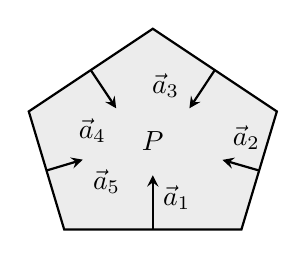
\begin{tikzpicture}[scale=1.5, >=stealth]
			% coordinates
			\coordinate (A) at (0,0);
			\coordinate (B) at (1.5,0);
			\coordinate (C) at (1.8,1);
			\coordinate (D) at (0.75,1.7);
			\coordinate (E) at (-0.3,1);
			% pentagon
			\filldraw[fill=gray!15, thick]
			(A) -- (B) -- (C) -- (D) -- (E) -- cycle;
		  % normal vectors
			% AB
			\draw[->, black, thick] (0.75,0) -- (0.75,0.46) node[below right] {$\vec{a}_1$};
			% BC
			\draw[->, black, thick] (1.65,0.5) -- (1.34,0.59) node[above right] {$\vec{a}_2$};
			% CD
			\draw[->, black, thick] (1.275,1.35) -- (1.06,1.027) node[above left] {$\vec{a}_3$};
			% DE
			\draw[->, black, thick] (0.225,1.35) -- (0.44,1.027) node[below left] {$\vec{a}_4$};
			% EA
			\draw[->, black, thick] (-0.15,0.5) -- (0.157,0.592) node[below right] {$\vec{a}_5$};
			% polyhedron label
			\node at (0.75, 0.75) {$P$};
		\end{tikzpicture}
	\end{minipage}
	\caption{\textit{Izquierda:} Un hiperplano afín $\braces{\vec{x} \colon \vec{a}^T\vec{x} = b}$
	junto con sus dos semi-espacios $\braces{\vec{x} \colon \vec{a}^T\vec{x} \geq \vec{b}}$ y
	$\braces{\vec{x} \colon \vec{a}^T\vec{x} \leq \vec{b}}$. \textit{Derecha:} Un politopo $P$.}
	\label{fig:hyp}
\end{figure}

\begin{definition}[\cite{fabs}]
	Sea $P \subseteq \R^n$ un poliedro. Decimos que el vector $\vec{x} \in P$ es un \textbf{vértice} de $P$ si existe
	$\vec{c} \in \R^n$ de manera que $\vec{c}^T\vec{x} < \vec{c}^T\vec{y}$ para todo $\vec{y} \in P
	\setminus \braces{\vec{x}}$.
\end{definition}

En términos gráficos, decimos que $\vec{x}$ es un vértice si se satisfacen dos condiciones: en
primer lugar, existe un hiperplano afín que pasa por $\vec{x}$ y uno de sus semi-espacios
contiene completamente al poliedro $P$; en segundo lugar, ningún otro punto de $P$ se encuentra
sobre este hiperplano.

\begin{definition}
Sea $P$ un poliedro y sea $\vec{c} \in \R^n$ un vector. Todo problema de optimización de la forma
\eqref{prim:lineal-opt} entra en una de las siguientes tres categorías:
\begin{enumerate}
	\item El valor óptimo no existe: ningún vector $\vec{x} \in \R^n$ satisface
		el sistema de desigualdades $A\vec{x} \geq \vec{b}$. Es decir, la región factible es vacía.
	\item El valor óptimo existe y es infinito: el poliedro $P$ no es acotado y
		existe una sucesión de vectores $\lbrace \vec{x}_k \rbrace_{k \in \N}$
		en el poliedro $P$ que satisface $\vec{c}^T\vec{x}_{k+1} > \vec{c}^T\vec{x}_k$ para todo $k \in \N$.
	\item El valor óptimo existe y es finito: este caso es la negación de los dos puntos anteriores.
		Observemos que aquí cabe la posibilidad de que el poliedro $P$ no sea acotado, pues puede
		que no exista la sucesión creciente de valores objetivo definida en el caso anterior.
\end{enumerate}
En el primer caso decimos que \textbf{el problema es infactible}, mientras que en los últimos dos
decimos que \textbf{el problema es factible}. También diremos comúnmente del segundo caso que
\textbf{el problema es no acotado}.
\end{definition}

En el capítulo 3 de \cite{fabs} se muestra que todo poliedro
\begin{equation*}
	P \coloneq \braces{\vec{x} \in \R^n \vcentcolon A\vec{x} \geq \vec{b}}
\end{equation*}
puede ser transformado a la forma estándar
\begin{equation*}
	\lbrace \left( \vec{x}^+, \vec{x}^-, \vec{s} \right) \in \R^{n + n + m} \vcentcolon A(\vec{x}^+ -
\vec{x}^-) - \vec{s} = \vec{b}, \left(\vec{x}^+, \vec{x}^-, \vec{s}\right) \geq \vec{0}\rbrace,
\end{equation*}
de manera que todo problema de optimización de la forma \eqref{prim:lineal-opt} puede ser escrito
sin pérdida de generalidad como
\begin{subequations}
	\label{prerreq:formulation}
	\begin{align}
		\max_{\vec{x} \in \R^n} \quad
			& \vec{c}^T\vec{x}, \label{prerreq:formulation:objective} \\
		\text{s.a.} \quad
			& A\vec{x} = \vec{b}, \label{prerreq:formulation:constraints} \\
			& \vec{x} \geq \vec{0} \nonumber.
	\end{align}
\end{subequations}
De ahora en adelante nuestro análisis se concentrará exclusivamente en problemas lineales en forma
estándar. A continuación enunciamos el teorema fundamental que nos permite resolver problemas
lineales.
\begin{theorem}
	\label{prerreq:th:linear-sol}
	Sea $P$ un poliedro que tiene al menos un vértice, consideremos el problema
	\eqref{prerreq:formulation}, y supongamos que el valor óptimo $z^*$ existe y es finito. Entonces
	el conjunto de soluciones óptimas contiene al menos un vértice de $P$.
\end{theorem}

Este teorema constituye el primer paso para la construcción de varios algoritmos que encuentran
soluciones del problema \eqref{prerreq:formulation}. El más famoso de todos es el algoritmo
\emph{simplex}, el cual ``salta'' de vértice en vértice hasta llegar a uno con valor óptimo. Otros,
más modernos y conocidos como \emph{métodos de puntos interiores}, comienzan en el interior del
poliedro $P$ y son ``atraídos'' como imanes a uno de los vértices con valor óptimo. No es el
objetivo de esta tesis exponer la teoría detrás de estos algoritmos. Sin embargo, al
lector interesado le recomendamos leer los capítulos 13 y 14 de \cite{nocedal}.

Ahora describimos brevemente los programas lineales enteros y explicamos el método de R\&A.
Supondremos en lo que resta de esta tesis que contamos con un algoritmo para resolver problemas
lineales.
\begin{definition}
	Sean $A \in \R^{m \times n}$ una matriz con renglones linealmente independientes, $\vec{c} \in
	\R^n$ un vector, y $\vec{b} \in \R^m$ otro vector. Al problema de optimización lineal
	\eqref{prerreq:formulation} lo llamamos \textbf{problema relajado} del \textbf{programa lineal
	entero}
	\begin{subequations}
		\label{prerreq:formulation:ilp}
		\begin{align}
			\max_{\vec{x} \in \Z^n} \quad
				& \vec{c}^T\vec{x}, \label{prerreq:formulation:objective:ilp} \\
			\text{s.a.} \quad
				& A\vec{x} = \vec{b}, \label{prerreq:formulation:constraints:ilp} \\
				& \vec{x} \geq \vec{0} \nonumber.
		\end{align}
	\end{subequations}
\end{definition}
Resalta el hecho de que la formulación de un programa lineal entero es idéntico a su formulación
relajada, y solamente intercambiamos nuestro espacio de búsqueda $\R^n$ por $\Z^n$. Es decir, lo único
que cambia es la región de factibilidad. De hecho, si definimos el poliedro
\begin{equation*}
	P \coloneq \lbrace \vec{x} \in \R^n \vcentcolon A\vec{x} = \vec{b}, \vec{x} \geq \vec{0} \rbrace,
\end{equation*}
entonces tenemos que $P \cap \Z^n$ corresponde a la región factible de
\eqref{prerreq:formulation:ilp}, mientras que $P$ corresponde a la región factible de su problema
relajado.

A partir de lo anterior, deducimos inmediatamente que el valor óptimo $z^*$ de un problema relajado
es una cota superior del valor óptimo $\optilp{z}$ de su programa lineal entero, pues ambos son
problemas de maximización y es cierto que $P \cap \Z^n \subseteq P$. De aquí se sigue que si
$\optilp{z} = z^*$, entonces la solución óptima $\vec{x}^*$ del problema relajado también es la
solución óptima del programa lineal entero si $\vec{x}^* \in \Z^n$.

Ramificación y Acotamiento encapsula una familia de métodos que comparten la misma estructura para
encontrar soluciones de programas lineales enteros. Específicamente, R\&A construye recursivamente
un árbol de subproblemas lineales relajados a resolver. Si la solución de un subproblema no es entera,
entonces su región factible es \textbf{ramificada} para generar otra colección de subproblemas y
cuyas soluciones podrían ser enteras. Es posible aplicar \textbf{criterios de poda} para eliminar
porciones del árbol que no contienen soluciones óptimas del problema original. Ilustramos el
procedimiento a través de un ejemplo concreto, en el cual enfatizamos estos componentes principales
que caracterizan a la familia de métodos.

% El algoritmo estándar para encontrar soluciones de programas lineales enteros es Ramificación y
% Acotamiento. Este método consiste en generar un árbol binario donde cada nodo representa un
% subproblema lineal a resolver. En la raíz del árbol resolvemos el problema relajado
% \eqref{prerreq:formulation} y, si la solución óptima $\vec{x}^* \in \R^n$ no es entera, entonces
% escogemos alguna entrada no entera $x_i^*$, creamos el nodo hijo izquierdo añadiendo la restricción
% $x_i \leq \floor{x_i^*}$ y también creamos el nodo hijo derecho añadiendo la restricción $x_i \geq
% \ceil{x_i^*}$. Este procedimiento se realiza de manera recursiva.
% 
% Observemos que, si decidimos recorrer todos los nodos del árbol binario, entonces tendremos que
% resolver al menos $2^n$ subproblemas, donde $n$ es la dimensión del problema lineal. Por esta razón,
% el algoritmo cuenta con políticas de poda para deshacerse de ramas cuyos nodos nunca proveerán la
% solución óptima. Ilustramos estas políticas a partir de un ejemplo.

\begin{example}[\cite{fabs}]
	\label{ex:ilp}
	Consideremos el programa lineal entero
	\begin{align*}
		\max_{(x_1, x_2) \in \Z^2} \quad
			& 4x_1 - x_2, \\
			\text{s.a.} \quad
			& 7x_1 - 2x_2 \leq 14, \\
			& 2x_1 - 2x_2 \leq 3, \\
			& x_2 \leq 3, \\
			& x_1, x_2 \geq 0.
	\end{align*}
	La región factible de este problema se muestra en la figura \ref{fig:feas} en la página
	\pageref{fig:feas}. La solución al problema
	relajado, cuya región factible denotamos por $S$, está dada por $\vec{x}^{(0)} \coloneq (20/7,
	3)$. Como $x_1^{(0)} = 20/7$ no es entero, \textbf{ramificamos binariamente} para generar los
	subproblemas con regiones factibles
	\begin{align*}
		S_{0} &\coloneq S \cap \braces{ (x_1, x_2) \in \R^2 \vcentcolon x_1 \leq \floor{20/7} = 2}, \\
		S_{1} &\coloneq S \cap \braces{ (x_1, x_2) \in \R^2 \vcentcolon x_1 \geq \ceil{20/7} = 3}.
	\end{align*}
	En este nivel del árbol así como en los siguientes, preferimos encontrar las soluciones de ambos
	subproblemas antes de ramificar cualesquiera de ellos. Es decir, realizamos una \textbf{búsqueda
	en anchura} (\textit{breadth-first search}) para resolver el problema original.

	Observamos en la figura \ref{fig:feas} que $S_{1}$ es vacío, así que no será posible
	ramificarlo. Ahora bien, la solución del problema con región factible $S_{0}$ es $\vec{x}^{(1)}
	\coloneq (2, 1/2)$. Puesto que $x_2^{(1)} = 1/2$ no es entero, ramificamos binariamente para
	generar los nuevos subproblemas con regiones factibles
	\begin{align*}
		S_{00} &\coloneq S_{0} \cap \braces{ (x_1, x_2) \in \R^2 \vcentcolon x_2 \leq \floor{1/2} = 0}, \\
		S_{01} &\coloneq S_{0} \cap \braces{ (x_1, x_2) \in \R^2 \vcentcolon x_2 \geq \ceil{1/2} = 1}.
	\end{align*}
	La solución $\vec{x}^{(2)}$ del subproblema con región factible $S_{01}$ es $(2, 1)$, y entonces
	es entera con valor objetivo $z_2^* \coloneq 7$. Decimos que esta solución es la
	\textbf{solución incumbente}: no vale la pena ramificar otros subproblemas cuyo valor objetivo
	sea menor o igual que $z_2^*$. En estos casos diremos que podamos esos subproblemas por
	\textbf{cota}. No es difícil ver que cualquier descendiente de $S_{01}$ será podado por cota.
	Además, observemos que la solución de $S_{00}$ es $\vec{x}^{(3)} \coloneq (3/2, 0)$, por lo que
	su valor objetivo es $6 < z_2*$, así que también podamos $S_{00}$ por cota.

	Como hemos agotado todos los subproblemas que podríamos explorar, concluimos que la solución
	óptima de este programa lineal entero es la única solución incumbente obtenida $\vec{x}^{(2)} =
	(2, 1)$ con valor objetivo 7.
\end{example}
\begin{figure}
	\centering
	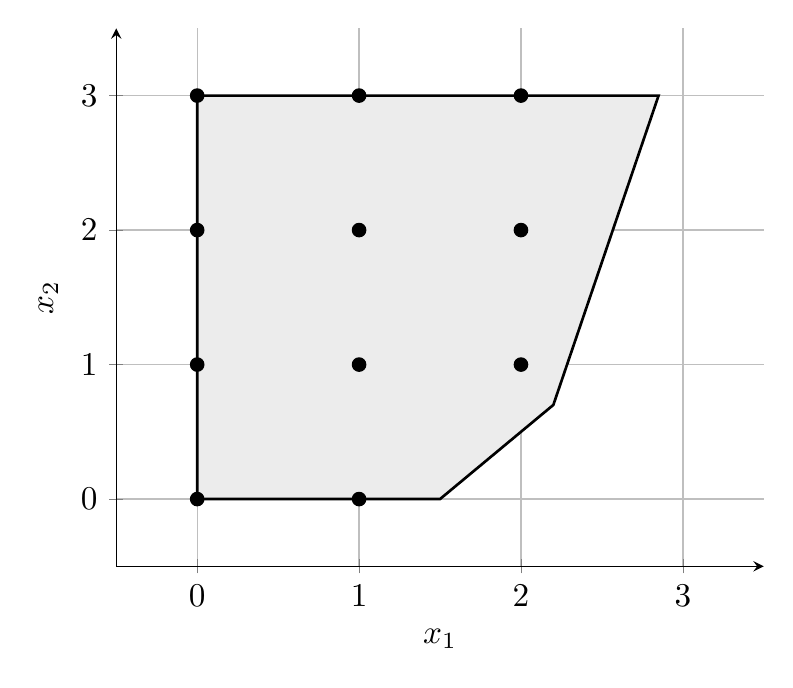
\begin{tikzpicture}[scale=1.2]
		\begin{axis}[
			axis lines=left,
			xmin=-0.5, xmax=3.5,
			ymin=-0.5, ymax=3.5,
			grid=both,
			xlabel=$x_1$,
			ylabel=$x_2$
			]
			\addplot+ [thick,color=black,fill=gray!15,mark=none] table {
				0 0
				1.5 0
				2.2 0.7
				2.85 3
				0 3
				0 3
				0 0
			};
			\addplot+ [only marks,,mark=*,mark options={scale=1, color=black, fill=black}] table {
				0 0
				0 1
				0 2
				0 3
				1 0
				1 1
				1 2
				1 3
				2 1
				2 2
				2 3
			};
		\end{axis}
	\end{tikzpicture}
	\caption{Los puntos negros forman la región factible del programa lineal entero del ejemplo
	\ref{ex:ilp}, mientras que la región sombreada es la región factible de su problema relajado.}
	\label{fig:feas}
\end{figure}

Como pudimos apreciar en este ejemplo, los componentes principales que caracterizan a Ramificación y
Acotamiento fueron la estrategia de búsqueda, que indica el orden en el que resolvemos los
subproblemas; la estrategia de ramificación, que indica cómo generar los descendientes de un nodo; y
las políticas de poda, que son reglas para eliminar subárboles de nuestra búsqueda. Estas tres
características están interrelacionadas: si hubiéramos resuelto el subproblema $S_{00}$ antes que
$S_{01}$, no habríamos tenido una solución incumbente, así que no lo habríamos podado y
entonces lo habríamos ramificado en otros dos subproblemas. En \cite{morrison} se recopilan avances
en estos tres componentes que constituyen líneas de investigación abiertas.

El algoritmo \ref{algo:bb2} en la página \pageref{algo:bb2} formaliza el procedimiento seguido en este
ejemplo, a excepción de la búsqueda en anchura, pero que es posible implementar con una fila
(\textit{queue}). En cuanto a los resultados teóricos que obtendremos a lo largo de esta tesis,
supondremos que nos referimos a este algoritmo en específico cuando hagamos mención genérica de
R\&A, y nos reservamos el calificativo de ``implementación pura'', pues es común que se enseñe esta
versión en cursos introductorios de investigación de operaciones. En cuanto a los resultados
numéricos, utilizaremos la implementación de código abierto \emph{COIN-OR Branch and Cut} (CBC) de
la fundación COIN-OR \cite{coin} para encontrar soluciones a programas lineales enteros. Otras
implementaciones comúnes de código abierto son HiGHS y SCIP, mientras que algunas implementaciones
comerciales son Gurobi Optimizer, IBM ILOG CPLEX Optimizer, y Fico Xpress Solver.

\begin{algorithm}[ht]
	\LinesNumbered
	\DontPrintSemicolon
	\KwData{
		Problema lineal relajado $S$.
		}
	\KwResult{
		Solución óptima entera $\vec{x}^*$ y valor óptimo $\optilp{z}$.
	}
	\Begin{
		$\mathcal{L} \leftarrow \braces{S}$\;
		$\vec{x}^* \leftarrow -\vec{\infty}$\;
		$\optilp{z} \leftarrow -\infty$\;
		\While{$\mathcal{L} \neq \emptyset$}{ \label{algo:bb:loop}
			elegir subproblema $S_i$\ de $\mathcal{L}$\quad\tcp*[h]{estrategia de búsqueda}\;
			obtener valor óptimo $z^*_i$ y solución óptima $\vec{x}^{(i)}$\ de $S_i$\;
			$\mathcal{L} \leftarrow \mathcal{L} \setminus \braces{S_i}$\;
			\If{$S_i = \emptyset$ o $z^*_i \leq \optilp{z}$}{
				\tcp*[h]{podar por cota}\;
				ir a la línea \ref{algo:bb:loop}\;
			}
			\If{$\vec{x}^{(i)} \in \Z^n$}{
				\tcp*[h]{solución incumbente}\;
				$\vec{x}^* \leftarrow \vec{x}^{(i)}$\;
				$\optilp{z} \leftarrow z^*_i$\;
				ir a la línea \ref{algo:bb:loop}\;
			}
			\tcp*[h]{ramificación binaria}\;
			elegir $x^{(i)}_j \not \in \Z$ y definir
			\begin{align*}
				S_{i0} \leftarrow S_{i} \cap \braces{\vec{x} \in \R^n \vcentcolon x_j \leq \lfloor x^{(i)}_j \rfloor}, \\
				S_{i1} \leftarrow S_{i} \cap \braces{\vec{x} \in \R^n \vcentcolon x_j \geq \lceil
				x^{(i)}_j \rceil}\;
			\end{align*}
			$\mathcal{L} \leftarrow \mathcal{L} \cup \braces{S_{i0}, S_{i1}}$.
		}
		\Return{$(\vec{x}^*, \optilp{z})$}
	}
	\caption{Ramificación y Acotamiento. Adaptado de \cite{fabs}.}
	\label{algo:bb2}
\end{algorithm}

\section{Fundamentos}
\label{sec:foundations}
\noindent
En primer lugar, se dan a conocer las definiciones y encunciados originalmente dados en \cite{herr}.
Es importante aclarar que se tradujeron los términos \textit{projectively rational
vectors} y \textit{c-layers} como ``vectores esencialmente enteros'' y ``capas enteras'' en las
definiciones \ref{theory:def:rational} y \ref{phase-1:def:c-layer}, respectivamente, a falta de
encontrar fuentes en español que hicieran uso de ellos.

En segundo lugar, se muestra una equivalencia entre resolver el programa lineal entero
\eqref{theory:formulation} y resolver ecuaciones lineales diofantinas. Este resultado se basa en los
teoremas \ref{prerreq:th:existence} y \ref{prerreq:th:construction} para construir inductivamente el
conjunto de soluciones de una ecuación lineal diofantina en $n$ incógnitas. Estas soluciones serán
definidas a partir de una relación de recurrencia y dependerán de una colección de $n - 1$
variables libres.

En tercer lugar, se exhibe una transformación lineal entre el conjunto de soluciones de una ecuación
lineal diofantina en $n$ incógnitas y el conjunto de $n - 1$ variables libres que determinan estas
soluciones. Luego, se investigan las propiedades de esta transformación lineal que serán de gran utilidad
teórica para los siguientes capítulos, en especial para el capítulo 4.

Finalmente, se muestra que el vector objetivo $\vec{p}$ del problema original
\eqref{theory:formulation} induce una descomposición de $\Z^n$ y se analiza cómo se relacionan las
descomposiciones asociadas a distintos vectores $\vec{p}$. Esto permitirá mostrar equivalencias
entre distintas instancias del problema \eqref{theory:formulation}.

\subsection{Capas enteras}
\label{subsec:sym}

\begin{definition}
	\label{theory:def:rational}
	Decimos que un vector $\vec{v} \in \R^n \setminus \lbrace \vec{0} \rbrace$ es
	\textbf{esencialmente entero} si existen un vector $\vec{w} \in \Z^n$ y un escalar $m \in \R
	\setminus \braces{0}$ tales que $\vec{v} = m\vec{w}$. Además, decimos que $\vec{w}$ es el
	\textbf{múltiplo coprimo} de $\vec{v}$ si sus entradas son coprimas y si su primera entrada no
	nula es positiva.
\end{definition}
\begin{example}
	El vector $\left(-\sqrt{2}, 1/\sqrt{2}\right) = 2\sqrt{2}(-2, 1)$ es esencialmente entero
	y $(2, -1)$ es su múltiplo coprimo. En contraste, el vector $\paren{\sqrt{2}, \sqrt{3}}$ no es
	esencialmente entero. Para ver esto último, supongamos que existe un escalar $m \in
	\R\setminus\braces{0}$ y enteros $a, b$ tales que $m(a, b) = \paren{\sqrt{2}, \sqrt{3}}$.
	Claramente, $a, b \neq 0$ y se debe cumplir $a/b = \sqrt{2/3}$, pero el lado izquierdo es un
	número racional mientras que el derecho es un número irracional, así que obtenemos una
	contradicción, por lo que el vector $\paren{\sqrt{2}, \sqrt{3}}$ no es esencialmente entero.
\end{example}
\begin{observation}
	\label{obs:coprime-unique}
	Todo vector $\vec{v}$ esencialmente entero tiene a lo más dos vectores coprimos asociados. Sean
	$m \in \R$ y $\vec{w} \in \Z^n$ tales que $\vec{v} = m\vec{w}$. Entonces
	\begin{equation*}
		\pm \frac{1}{\gcd{w_1, \ldots, w_n}}\vec{w}
	\end{equation*}
	son dos vectores cuyas entradas son coprimas, de acuerdo al lema \ref{prerreq:lemma:gcd}. Como
	la primera entrada no nula $w_i$ también debe ser positiva, se sigue que solo uno de estos dos
	vectores es el múltiplo coprimo de $\vec{v}$. Así, el múltiplo coprimo de un vector
	esencialmente entero es único.
\end{observation}
\begin{observation}
	Todo vector racional $\vec{v} \in \Q^n \setminus \braces{\vec{0}} $  es esencialmente
	entero. En efecto, para cada $i \in \braces{1, \ldots, n}$ existen $p_i, q_i \in
	\Z$ con $q_i \neq 0$ tales que $v_i = p_i/q_i$. Luego, si definimos $m \coloneq \lcm{q_1,
	\ldots, q_n} \neq 0$ y también $\vec{w} \coloneq m\vec{v} \in \Z^n$, encontramos que $\vec{v} =
	\frac{1}{m}\vec{w}$.
\end{observation}

% Desde el punto de
% vista puramente teórico, esta condición reduce de manera drástica el tipo de programas lineales que
% podemos resolver. No obstante, esta clase de vectores es un poco más general que los considerados en
% otros textos de programación lineal. Por ejemplo, \cite{martello} y \cite{alex} toman en cuenta
% vectores puramente racionales.

\begin{definition}
	\label{phase-1:def:c-layer}
	Sea $\vec{v} \in \R^n$ un vector esencialmente entero y sea $t \in \R$ un escalar. Decimos que
	su hiperplano afín asociado
	\begin{equation}
		\label{phase-1:def:affine-hyperplane}
		\clayer{\vec{v}}{t} \coloneq \ker{\vec{x} \mapsto \vec{v}^T\vec{x}} + t\vec{v}
		= \lbrace \vec{v}^{\perp} + t\vec{v} \vcentcolon \vec{v}^T\vec{v}^{\perp} = 0 \rbrace
	\end{equation}
	es una \textbf{capa entera} si contiene al menos un punto entero.
\end{definition}

La ventaja principal de utilizar la clase de vectores esencialmente enteros en vez de los vectores
sobre $\R^n$ o sobre $\Q^n$ se debe a que esta clase es la más grande, de acuerdo al teorema 9 de
\cite{herr}, en la que el número de capas enteras es finita entre cualesquiera dos puntos. Los
algoritmos que presentaremos en el capítulo 3 enumeran estas capas enteras, así que su finitud
asegura la terminación en tiempo finito de estos algoritmos.

\begin{lemma}
	\label{phase-1:lemma:layer}
	Sean $\vec{v}, \vec{x} \in \R^n$ con $\vec{v}$ distinto de cero. Entonces $\vec{x} \in
	\clayer{\vec{v}}{t_{\vec{x}}}$, donde $t_{\vec{x}} \coloneq
	\frac{\vec{v}^T\vec{x}}{\norm{\vec{v}}^2}$.
\end{lemma}

Las capas enteras son invariantes ante reescalamientos en el vector $\vec{v}$: si $r \neq 0$,
entonces $\clayer{\vec{v}}{t} = \clayer{r\vec{v}}{t/r}$. Esta igualdad se prueba por contenciones.
Sea $\vec{x} \in \clayer{\vec{v}}{t}$, entonces existe $\vec{v}^\perp$ ortogonal a $\vec{v}$ tal que
\begin{equation*}
	\vec{x} = \vec{v}^\perp + t\vec{v} = \vec{v}^\perp + \frac{t}{r}(r\vec{v}).
\end{equation*}
Pero si $\vec{v}^\perp$ es ortogonal a $\vec{v}$, entonces también es ortogonal a $r\vec{v}$. Así,
encontramos que $\vec{x} \in \clayer{r\vec{v}}{t/r}$. La otra contención se muestra de manera
similar.

En particular, si $\vec{w}$ es el múltiplo coprimo de $\vec{v}$, se cumple que
\begin{equation}
	\label{eq:clayer-eq}
	\braces{\clayer{\vec{v}}{t} \vcentcolon t \in \R}
	=
	\braces{\clayer{\vec{v}/m}{t m} \vcentcolon t \in \R}
	=
	\braces{\clayer{\vec{w}}{t} \vcentcolon t \in \R},
\end{equation}
donde $m \neq 0$ es el escalar que satisface $\vec{v} = m\vec{w}$. Así pues, para analizar las capas
enteras, basta con fijarnos en los múltiplos coprimos que las definen en vez de sus vectores
esencialmente enteros asociados.

\begin{theorem}
	\label{phase-1:th:cover}
	Sea $\vec{v} \in \R^n$ un vector esencialmente entero y sea $\vec{w}$ su múltiplo coprimo.
	Entonces una cobertura de $\Z^n$ está dada por la familia de capas enteras
	$\braces{\qlayer{w}{k} \vcentcolon k \in \Z}$.
\end{theorem}

\begin{lemma}
	\label{theory:lemma:utility}
	Sea $\vec{v} \in \R^n$ un vector esencialmente entero y sea $\vec{w}$ su múltiplo coprimo.
	Entonces $\vec{w}^T\vec{x} = k$ para todo $\vec{x} \in \qlayer{w}{k}$.
\end{lemma}
\begin{proof}
	Sea $\vec{x} \in \qlayer{w}{k}$, por lo que existe un vector $\vec{w}^\perp$ ortogonal a
	$\vec{w}$ tal que
	\begin{equation*}
		\vec{x} = \vec{w}^\perp + \frac{k}{\norm{\vec{w}}^2}\vec{w}.
	\end{equation*}
	Luego,
	\begin{equation*}
		\vec{w}^T\vec{x} = \vec{w}^T\vec{w}^\perp + \frac{k}{\norm{\vec{w}}^2}\vec{w}^T\vec{w}
		=
		0 + \frac{k}{\norm{\vec{w}}^2}\norm{\vec{w}}^2 = k.
	\end{equation*}
	que es lo que deseábamos obtener.
\end{proof}

% Pasemos a considerar el programa lineal (\ref{theory:formulation}) donde $\vec{p}$ es un vector
% esencialmente entero y $\vec{q}$ es su múltiplo coprimo. Comúnmente a la función objetivo
% (\ref{theory:objective}) le daremos el nombre de utilidad y a la restricción
% (\ref{theory:constraint:budget}) la llamaremos restricción presupuestaria, así como presupuesto al
% lado derecho de esta restricción.

Supongamos que el vector objetivo $\vec{p}$ del problema \eqref{theory:formulation} es esencialmente
entero y sea $\vec{q}$ su múltiplo coprimo. Puesto que el espacio de búsqueda de este problema es
$\Z^n$, se sigue de \eqref{eq:clayer-eq} y del teorema \ref{phase-1:th:cover} que podemos
restringir la búsqueda a la familia de capas enteras $\braces{\qlayer{q}{k} \vcentcolon k \in \Z}$.

Del lema \ref{theory:lemma:utility} encontramos que los puntos de la \textbf{$k$-ésima capa entera}
o bien respetan todos la restricción presupuestaria \eqref{theory:constraint:budget}, o bien ninguno
lo hace. Sea $\vec{x} \in \qlayer{q}{k}$ y observemos que
\begin{equation}
	\label{eq:eta-cases}
	\vec{p}^T\vec{x} = m\vec{q}^T\vec{x} = mk \leq u
	\iff
	\begin{cases}
		k \geq u/m, & m < 0, \\
		k \leq u/m, & m > 0,
	\end{cases}
\end{equation}
donde $m \neq 0$ es el escalar que satisface $\vec{p} = m\vec{q}$. Obtenemos de manera inmediata el
siguiente lema.
% Así pues, dependiendo del signo de $m$, tenemos que el primer parámetro $\eta$ en satisfacer la
% restricción presupuestaria puede ser interpretado como el entero más pequeño o el entero más grande
% que satisface su respectiva desigualdad.

\begin{lemma}
	\label{phase-1:lemma:eta}
	Sea $\vec{p} \in \R^n$ un vector esencialmente entero y sea $\vec{q}$ su múltiplo coprimo, de
	manera que $\vec{p} = m\vec{q}$ para algún escalar $m \neq 0$. Entonces la primera capa entera
	$\qlayer{q}{\eta}$ en satisfacer la restricción \eqref{theory:constraint:budget} está
	parametrizada por
	\begin{equation}
		\label{lemma:eq:eta-cases}
		\eta \coloneq \begin{cases}
			\ceil{u/m}, & m < 0, \\
			\floor{u/m}, & m > 0.
		\end{cases}
	\end{equation}
\end{lemma}

Puesto que la gran mayoría de nuestros enunciados y algoritmos dependen del parámetro
$\eta$, tendremos que separarlos al menos en dos casos. Creemos que es prudente
considerar solamente el caso $m > 0$, ya que los enunciados y demostraciones para
el caso $m < 0$ son completamente análogos. Las diferencias recaen, por ejemplo, en que el orden de
las desigualdades cambian o las funciones piso se reemplazan por funciones techo.

En resumen, si $m > 0$, encontramos que las capas enteras que satisfacen la restricción
\eqref{theory:constraint:budget} están parametrizadas por $k \in \braces{\eta, \eta - 1, \ldots}$.
Además, por el lema \ref{theory:lemma:utility}, todo $\vec{x} \in \qlayer{q}{k}$ satisface la
ecuación $\vec{q}^T\vec{x} = k \leq \eta \leq u$, donde $u$ es el lado derecho de la restricción
\eqref{theory:constraint:budget}.
\begin{theorem}
	\label{theory:th:infeasibility}
	Sea $\vec{p} \in \R^n$ un vector esencialmente entero y sea $\vec{q}$ su múltiplo coprimo.
	Entonces el problema \eqref{theory:formulation} es infactible si y solo si $\vec{q} \geq
	\vec{0}$ y el lado derecho $u$ de la restricción \eqref{theory:constraint:budget} es negativo. 
\end{theorem}
\begin{proof}
	$(\implies)$ Supongamos que $\vec{q} \geq \vec{0}$ y $u < 0$. Si $\vec{x} \in \Z_{\geq
	\vec{0}}^n$ entonces $\vec{q}^T\vec{x} \geq 0 > u$ y por lo tanto $\vec{x}$ no es factible.
	Luego,
	\begin{equation*}
		\Z_{\geq \vec{0}}^{n} \cap \lbrace \vec{x} \vcentcolon \vec{q}^T\vec{x} 
		\leq u \rbrace = \emptyset,
	\end{equation*}
	y el problema no es factible.

	$(\impliedby)$ Procedemos por contraposición. Si $u
	\geq 0$ observamos que $\vec{0} \in \Z^n$ es factible. Se debe cumplir $u < 0$. Similarmente, si
	$q_i < 0$ para algún $i \in \lbrace 1, \ldots, n \rbrace$, encontramos que $\lceil u/q_i
	\rceil\vec{e}_i \in \Z^n$ es factible:
	\begin{equation*}
		\vec{q}^T\left\lceil \frac{u}{q_i} \right\rceil\vec{e}_i
		= q_i \left\lceil \frac{u}{q_i} \right\rceil
		\leq q_i \frac{u}{q_i} = u,
	\end{equation*}
	además, como $u < 0$, concluimos que $\lceil u/q_i \rceil\vec{e}_i$ es no negativo.
\end{proof}

Debido al teorema anterior, somos capaces de determinar automáticamente si el problema
\eqref{theory:formulation} es infactible, por lo que supondremos de ahora en adelante que es
factible. El siguiente teorema muestra que nuestro análisis para resolver este problema debe
dividirse en dos casos.

\begin{theorem}
	\label{theory:th:feasibility}
	Sea $\vec{p} \in \R^n$ un vector esencialmente entero y sea
	$\vec{q}$ su múltiplo coprimo, de manera que $\vec{p} = m\vec{q}$ para alguna $m > 0$.
	Supongamos que el problema \eqref{theory:formulation} es factible y tomemos $\eta$ del lema
	\ref{phase-1:lemma:eta}. Entonces se satisface lo siguiente: \begin{enumerate}
		\item Si $q_i < 0$ para algún $i \in \braces{1, \ldots, n}$, entonces la $\eta$-ésima
			capa entera $\qlayer{q}{\eta}$ contiene un número infinito de puntos factibles.
		\item Si $\vec{q} > \vec{0}$ entonces, para todo $k \in \braces{\eta, \eta - 1, \ldots, 0}$,
			la $k$-ésima capa entera $\qlayer{q}{k}$ contiene un número finito de puntos factibles.
	\end{enumerate}
\end{theorem}
\begin{proof} \hfill
	\begin{enumerate}
		\item
			En la subsección \ref{subsec:dioph-eq} mostraremos que, como $\vec{q}$ es un vector
			coprimo, entonces existe un punto entero $\vec{x}$ que satisface la
			ecuación lineal diofantina $\vec{q}^T\vec{x} = \eta$. Por el momento confiemos que esto
			es verdadero. Luego,
			\begin{equation*}
				\vec{p}^T\vec{x} = m\vec{q}^T\vec{x} = m\eta = m\floor{\frac{u}{m}} \leq
				m\frac{u}{m} = u,
			\end{equation*}
			y se satisface la restricción \eqref{theory:constraint:budget}.

			Como no tenemos asegurada la no negatividad de $\vec{x}$, construiremos un vector entero
			$\vec{x}^+$ que sí satisface la restricción de no negatividad y también la restricción
			presupuestaria $\vec{q}^T\vec{x}^+ = \eta$, de manera que $\vec{x}^+$ sí será factible.

			Definamos los siguientes conjuntos de índices:
			\begin{equation*}
				I^+ \coloneq \lbrace i \vcentcolon q_i > 0 \rbrace,
				\quad I^\circ \coloneq \lbrace \ell \vcentcolon q_\ell = 0 \rbrace.
				\quad I^- \coloneq \lbrace j \vcentcolon q_j < 0 \rbrace.
			\end{equation*}
			Podemos suponer sin pérdida de generalidad que $I^\circ$ es vacío. En efecto, si $x_k
			< 0$ para alguna $k \in I^\circ$, esa entrada no sería factible, pero fácilmente
			podríamos definir $x_k^+ = 0$ para hacerla factible.

			Por hipótesis, sabemos que $\vec{q}$ tiene una entrada negativa y por lo tanto $I^- \neq
			\emptyset$. Además, por la definición \ref{theory:def:rational}, $\vec{q}$ tiene una
			entrada positiva y por lo tanto $I^+ \neq \emptyset$. Luego, ambos conjuntos $I^+$ e
			$I^-$ forman una partición del conjunto $\braces{1, \ldots, n}$. Podemos escoger
			enteros positivos $\braces{c_i}_{i \in I^+}$ que satisfagan simultáneamente
			\begin{align}
				x_k + \sum_{i \in I^+}q_ic_i &\geq 0, \quad \forall k \in I^-,
				\label{theory:pf:1} \\
				x_k - \sum_{j \in I^-}q_jc_k &\geq 0, \quad \forall k \in I^+.
				\label{theory:pf:2}
			\end{align}
			Definamos el vector $\vec{x}^+ \in \Z^n$ de manera que
			\begin{equation*}
				x^+_k \coloneq \begin{cases}
					x_k + \sum_{i \in I^+}q_ic_i, \quad k \in I^-, \\
					x_k - \sum_{j \in I^-}q_jc_k, \quad k \in I^+.
				\end{cases}
			\end{equation*}
			Se verifica que $\vec{x}^+$ es no negativo y, además,
			\begin{align*}
				\vec{q}^T\vec{x}^+
				&= \vec{q}^T\vec{x}
				+ \sum_{k \in I^-}\sum_{i \in I^+}q_kq_ic_i
				- \sum_{k \in I^+}\sum_{j \in I^-}q_kq_jc_k \\
				&= \eta
				+ \sum_{j \in I^-}\sum_{i \in I^+}q_jq_ic_i
				- \sum_{i \in I^+}\sum_{j \in I^-}q_iq_jc_i \\
				&= \eta.
			\end{align*}
			Así pues, tenemos existencia de un punto factible. Para concluir que hay un número
			infinito de puntos factibles, basta observar que si la elección de coeficientes
			$\braces{c_i}_{i \in I^+}$ satisface ambas desigualdades \eqref{theory:pf:1} y \eqref{theory:pf:2},
			entonces cualquier múltiplo entero positivo de estos coeficientes también las satisface.
		\item Se sigue del teorema anterior que $u \geq 0$. Definamos
			\begin{equation}
				\label{theory:pf:p_k}
				P_k \coloneq \paren{\qlayer{q}{k} \cap \Z_{\geq \vec{0}}^n}
				= \left\lbrace \vec{x} \in \Z^n \vcentcolon \vec{q}^T\vec{x} = k,
					\vec{x} \geq \vec{0} \right\rbrace,
			\end{equation}
			y observemos que $P_k = \emptyset$ para todo $k$ negativo, pues $\vec{q} > \vec{0}$ y por
			lo tanto $\vec{q}^T\vec{x} \geq 0$ para cualquier $\vec{x} \in \Z^n_{\geq \vec{0}}$. Esto implica que
			ningún punto sobre capas enteras con parámetros negativos es factible.

			Sea $k \in \braces{\eta, \eta - 1, \ldots, 0}$. La capa entera $\qlayer{q}{k}$
			interseca los ejes positivos en $\frac{k}{q_i}\vec{e}_i$,
			así que definamos $\ell_i \coloneq \lceil k/q_i \rceil$. Luego,
			\begin{equation*}
				\qlayer{q}{k} \cap \R^n_{\geq \vec{0}} \subseteq \prod_{i = 1}^{n} [0, \ell_i],
			\end{equation*}
			pues del caso contrario podemos escoger $\vec{x} \in \qlayer{q}{k}$ con $\vec{x} \geq
			\vec{0}$ y también $x_i > \ell_i$ para alguna $i \in \braces{1, \ldots, n}$. Por el lema
			\ref{theory:lemma:utility} tenemos
			\begin{equation*}
				k = \vec{q}^T\vec{x} > \sum_{j \neq i}q_jx_j + q_i\ceil{\frac{k}{q_i}}
			\end{equation*}
			y entonces
			\begin{equation*}
				0 \geq k - q_i\ceil{\frac{k}{q_i}} > \sum_{j \neq i}q_jx_j \geq 0.
			\end{equation*}
			De donde la última desigualdad se obtiene del hecho que ambos $\vec{q}$ y $\vec{x}$ son
			no negativos. Así pues, obtenemos una contradicción y la contención anterior es cierta.
			De esta manera, obtenemos
			\begin{equation*}
				\paren{\qlayer{q}{k} \cap \R^n_{\geq \vec{0}}} \cap \Z^n_{\geq \vec{0}} = P_k
				\subseteq \paren{\prod_{i = 1}^{n} [0, \ell_i]} \cap \Z^n = \prod_{i = 1}^{n}
				\left( [0, \ell_i] \cap \Z \right).
			\end{equation*}
			Pero $\left| [0, \ell_i] \cap \Z \right| = \ell_i + 1$. Así,
			\begin{equation*}
				|P_k| \leq \prod_{i = 1}^{n} (\ell_i + 1) < \infty.
			\end{equation*}
			Entonces la $k$-ésima capa entera contiene un número finito de puntos factibles.
	\end{enumerate}
\end{proof}

% Así pues, suponiendo que el problema \eqref{theory:formulation} tiene solución, el teorema
% \ref{theory:th:feasibility} nos sugiere dividir nuestro análisis en dos casos: uno donde una
% entrada $p_i$ es negativa y por lo tanto existe una infinidad de soluciones en la $\eta$-ésima
% capa entera; y uno donde $\vec{p}$ es estrictamente positivo, lo que implica la finitud de puntos
% factibles.

Ciertamente el primer caso del teorema \ref{theory:th:feasibility} es el menos interesante, pues
conocemos inmediatamente el valor óptimo de estas instancias. No obstante, existen muchos elementos
en común que comparten ambos casos. También es cierto que esta división dejará de existir una vez
que introduzcamos múltiples restricciones en el capítulo 4.

Además, antes de analizar los dos casos que el teorema anterior impone, primero debemos mostrar que la
ecuación lineal diofantina $\vec{q}^T\vec{x} = k$ admite soluciones enteras para toda $k \in \Z$
siempre que las entradas de $\vec{q}$ sean coprimas. Habíamos supuesto esto en la demostración
anterior.

Así también, la construcción de soluciones enteras de ecuaciones lineales diofantinas proveerá
herramientas teóricas útiles para demostrar la gran mayoría de resultados que presentaremos. Por lo
tanto, la siguiente subsección se encarga de construir solamente soluciones enteras de estas
ecuaciones. Será cuestión de los capítulos 2 y 3 obtener soluciones sean no negativas.

\subsection{Construcción de soluciones enteras}
\label{subsec:dioph-eq}
\noindent
Debido al teorema \ref{phase-1:th:cover}, las soluciones del problema \eqref{theory:formulation} se
encuentran en una capa entera $\qlayer{q}{k}$. Luego, por el lema \ref{theory:lemma:utility}, los
puntos $\vec{x} \in \Z^n$ que se encuentran sobre esa capa satisfacen la ecuación lineal diofantina
\begin{equation}
	\label{eq:dioph}
	\vec{q}^T\vec{x} = q_1x_1 + q_2x_2 + \cdots + q_nx_n = k.
\end{equation}
con $\vec{q} = (q_1, \ldots, q_n)$. Como hemos mencionado previamente, podemos suponer sin pérdida
de generalidad que ninguna entrada de $\vec{q}$ es nula.

En la sección \ref{section:number-theory} mostramos condiciones de existencia
de este tipo de ecuaciones, así como su construcción, cuando $n = 2$. Partimos de la
observación que podemos resolver recursivamente esta ecuación. Definamos, por conveniencia, $g_1
\coloneq \gcd{q_1, \ldots, q_n}$ y también $\omega_1 \coloneq k$. Puesto que $\vec{q}$ es un vector
con entradas coprimas, sabemos que $g_1 = 1$. También definamos
\begin{equation}
	\label{def:dummy:omega-2}
	\omega_2 \coloneq \frac{q_2}{g_2 \cdot g_1}x_2 + \cdots + \frac{q_n}{g_2 \cdot
	g_1}x_n,
\end{equation}
donde $g_2 \coloneq \gcd{q_2/g_1, \ldots, q_n/g_1}$. Como $q_n \neq 0$, tenemos que $g_2$ está bien
definido y además es positivo. Así, la ecuación \eqref{eq:dioph} es equivalente a
\begin{equation}
	\label{eq:dioph:first-step}
	\frac{q_1}{g_1}x_1 + g_2\omega_2 = \omega_1.
\end{equation}
Observemos que
\begin{align*}
	\gcd{\frac{q_1}{g_1}, g_2}
	&= \gcd{\frac{q_1}{g_1}, \gcd{\frac{q_2}{g_1}, \ldots, \frac{q_n}{g_1}}} \\
	&= \gcd{\frac{q_1}{g_1}, \frac{q_2}{g_1}, \ldots, \frac{q_n}{g_1}} = 1.
\end{align*}
Por el teorema \ref{prerreq:th:existence}, existen soluciones enteras para todo $\omega_1 \in \Z$.
Como $q_1/g_1$ y $g_2$ son coprimos, encontramos que sus coeficientes de Bézout (ver definición
\ref{prerreq:def:bezout}) asociados $x_1', \omega_2'$ son soluciones particulares de la ecuación
\begin{equation*}
	\frac{q_1}{g_1}x_1' + g_2\omega_2' = 1.
\end{equation*}
Deducimos del teorema \ref{prerreq:th:construction} que las soluciones de la ecuación
\eqref{eq:dioph:first-step} están dadas por
\begin{equation}
	\label{dummy:eq:first-step}
	\begin{cases}
		x_1 = \omega_1x_1' + g_2t_1, \\
		\omega_2 = \omega_1\omega_2' - \frac{q_1}{g_1}t_1,
	\end{cases}
\end{equation}
donde $t_1 \in \Z$ es una variable libre.

\begin{observation}
	Los coeficientes de Bézout $x_1'$ y $\omega_2'$ dependen exclusivamente de $\vec{q}$ y no del
	punto $\vec{x}$. En efecto, $x_1'$ está asociado a $q_1/g_1$ y $\omega_2'$ está asociado a
	$g_2$. Pero ambos $g_1$ y $g_2$ son el máximo común divisor de $q_1, \ldots q_n$ y de
	$q_1/g_1, \ldots, q_n/g_1$, respectivamente. 
\end{observation}

Para el siguiente paso de la recursión, escogemos cualquier $t_1 \in \Z$ para fijar $\omega_2$.
Tenemos de \eqref{def:dummy:omega-2} que debemos resolvemos la ecuación
\begin{equation}
	\label{eq:dioph:second-step}
	\frac{q_2}{g_2 \cdot g_1}x_2 +
	\frac{q_3}{g_2 \cdot g_1}x_3 +
	\cdots +
	\frac{q_n}{g_2 \cdot g_1}x_n
	= \omega_2.
\end{equation}
Como $g_2 = \gcd{q_2/g_1, \ldots, q_n/g_1}$, sabemos del lema \ref{prerreq:lemma:gcd}
que
\begin{equation*}
	\gcd{\frac{q_2}{g_2 \cdot g_1}, \ldots, \frac{q_n}{g_2 \cdot g_1}} = 1.
\end{equation*}
En el mismo espíritu del primer paso de la recursión, definimos
\begin{equation*}
	\omega_3 \coloneq \frac{q_3}{g_3 \cdot g_2 \cdot g_1}x_3 + \cdots + \frac{q_n}{g_3
	\cdot g_2 \cdot g_1}x_n,
\end{equation*}
donde
\begin{equation*}
	g_3 \coloneq  \gcd{\frac{q_3}{g_2 \cdot g_1}, \ldots, \frac{q_n}{g_2 \cdot g_1}}.
\end{equation*}
Nuevamente, como $q_n$ es distinto de cero, $g_3$ está bien definido y además es positivo. Así pues,
la ecuación \eqref{eq:dioph:second-step} es equivalente a
\begin{equation}
	\label{eq:dioph:second-step:short}
	\frac{q_2}{g_2 \cdot g_1}x_2 + g_3\omega_3 = \omega_2.
\end{equation}
También se cumple que
\begin{equation*}
	\gcd{\frac{q_2}{g_2 \cdot g_1}, g_3} = 1,
\end{equation*}
y entonces \eqref{eq:dioph:second-step:short} tiene una infinidad de soluciones para todo $\omega_2 \in
\Z$, las cuales están dadas por
\begin{equation*}
	\begin{cases}
		x_2 = \omega_2x_2' + g_3t_2, \\
		\omega_3 = \omega_2\omega_3' - \frac{q_2}{g_2 \cdot g_1}t_2,
	\end{cases}
\end{equation*}
donde $t_2 \in \Z$ es una variable libre, y $x_2', \omega_3'$ son los coeficientes de Bézout
asociados a $\frac{q_2}{g_2 \cdot g_1}$ y $g_3$, respectivamente.

De manera general, para $i \in \lbrace 1, \ldots, n - 2 \rbrace$, el $i$-ésimo paso de la recursión
provee la ecuación
\begin{equation}
	\label{dummy:eq:ith-equation}
	\frac{q_i}{\prod_{j=1}^{i}g_j}x_i
	+ \frac{q_{i+1}}{\prod_{j=1}^{i}g_j}x_{i+1}
	+ \cdots
	+ \frac{q_{n}}{\prod_{j=1}^{i}g_j}x_n
	= \omega_i,
\end{equation}
donde
\begin{equation}
	\label{dummy:eq:ith-g}
	g_i \coloneq \gcd{\frac{q_i}{\prod_{j=1}^{i-1}g_j}, \ldots, \frac{q_n}{\prod_{j=1}^{i-1}g_j}},
\end{equation}
por el lema \ref{prerreq:lemma:gcd} se sigue que
\begin{equation}
	\label{dummy:coprime}
	\gcd{\frac{q_i}{\prod_{j=1}^{i}g_j}, \ldots, \frac{q_n}{\prod_{j=1}^{i}g_j}} = 1.
\end{equation}
Ahora bien, definamos
\begin{equation}
	\label{dummy:next-g}
	g_{i + 1} \coloneq \gcd{
		\frac{q_{i+1}}{\prod_{j=1}^{i}g_j},
		\ldots,
		\frac{q_{n}}{\prod_{j=1}^{i}g_j}
	}.
\end{equation}
Como $q_n$ es distinto de cero, se sigue que $g_{i + 1}$ está bien definido y es positivo.
Definamos
\begin{equation*}
	\omega_{i+1} \coloneq
	\frac{q_{i+1}}{\prod_{j=1}^{i + 1}g_j}x_{i+1}
	+ \cdots +
	\frac{q_{n}}{\prod_{j=1}^{i + 1}g_j}x_{n},
\end{equation*}
de manera que la ecuación \eqref{dummy:eq:ith-equation} es equivalente a
\begin{equation}
	\label{dummy:eq:simplified}
	\frac{q_i}{\prod_{j=1}^{i}g_j}x_i + g_{i+1}\omega_{i+1} = \omega_i.
\end{equation}
A partir de \eqref{dummy:coprime} y de \eqref{dummy:next-g}, encontramos que
\begin{align*}
	\gcd{
		\frac{q_i}{\prod_{j=1}^{i}g_j},
		g_{i+1}
	}
	&=
	\gcd{
		\frac{q_i}{\prod_{j=1}^{i}g_j},
		\frac{q_{i+1}}{\prod_{j=1}^{i}g_j},
		\ldots,
		\frac{q_n}{\prod_{j=1}^{i}g_j}
	} = 1,
\end{align*}
y del teorema \ref{prerreq:th:existence} se sigue que la ecuación \eqref{dummy:eq:simplified}
tiene soluciones enteras para todo $\omega_i \in \Z$. Por el teorema \ref{prerreq:th:construction},
las soluciones enteras de \eqref{dummy:eq:simplified} están dadas por
\begin{equation}
	\label{eq:recurrence}
	\begin{cases}
		x_i = \omega_ix_i' + g_{i + 1}t_i, \\
		\omega_{i + 1} = \omega_i\omega_{i + 1}' - \frac{q_i}{\prod_{j=1}^{i}g_j}t_i,
	\end{cases}
\end{equation}
donde $t_i \in \Z$ es la $i$-ésima variable libre. Es valioso mencionar, otra vez, que los
coeficientes de Bézout $x_i', \omega_{i+1}'$ dependen exclusivamente de $\vec{q}$ a través de sus
entradas $q_i$ y de los máximos común divisores entre ellas. En efecto, por el teorema
\ref{prerreq:th:bezout}, estos coeficientes son soluciones particulares de la ecuación
\begin{equation}
	\label{dummy:eq:bez-eq}
	\frac{q_i}{\prod_{j=1}^{i}g_j}x_i' + g_{i+1}\omega_{i+1}' = 1.
\end{equation}

Finalmente, en el último paso de la recursión obtenemos la ecuación lineal diofantina
\begin{equation}
	\label{eq:last-equation}
	\frac{q_{n-1}}{\prod_{j=1}^{n-1}g_j}x_{n-1} +
	\frac{q_{n}}{\prod_{j=1}^{n-1}g_j}x_n
	= \omega_{n-1}.
\end{equation}
Por construcción, los coeficientes de $x_{n - 1}$ y $x_n$ son coprimos. A causa del teorema
\ref{prerreq:th:construction} las soluciones enteras están dadas por
\begin{equation}
	\label{eq:last-solution}
	\begin{cases}
		x_{n-1} = \omega_{n-1}x_{n-1}' + \frac{q_n}{\prod_{j=1}^{n-1}g_j}t_{n-1}, \\
		x_n = \omega_{n-1}x_n' - \frac{q_{n-1}}{\prod_{j=1}^{n-1}g_j}t_{n-1},
	\end{cases}
\end{equation}
donde $x_{n-1}', x_n'$ son los coeficientes de Bézout asociados a
$\frac{q_n}{\prod_{j=1}^{n-1}g_j}$ y $\frac{q_{n-1}}{\prod_{j=1}^{n-1}g_j}$,
respectivamente, por lo que satisfacen
\begin{equation}
	\label{eq:last-equation-bez}
	\frac{q_{n-1}}{\prod_{j=1}^{n-1}g_j}x_{n-1}' +
	\frac{q_{n}}{\prod_{j=1}^{n-1}g_j}x_n'
	= 1.
\end{equation}

Hemos demostrado, que la ecuación lineal diofantina \eqref{eq:dioph} tiene al menos una solución,
siempre que $\vec{q}$ sea un vector coprimo. Así pues, saldamos nuestra cuenta pendiente con
respecto a una parte de la demostración \ref{theory:th:feasibility}. Además, construimos una
infinidad de soluciones enteras, pues la elección de cada variable libre $t_i \in \Z$ provee una
solución distinta. Aún más, por el teorema \ref{prerreq:th:construction}, sabemos que el conjunto de
estas soluciones es exhaustiva. En la siguiente subsección estableceremos, a partir de
la construcción de soluciones aquí obtenida, una relación lineal entre las soluciones enteras
$\vec{x} = (x_1, \ldots, x_n)$ de la ecuación lineal diofantina $\vec{q}^T\vec{x} = k$ y el vector
de variables libres $\vec{t} = (t_1, \ldots, t_{n-1})$.

Con respecto a la no negatividad de las soluciones mencionamos brevemente lo siguiente.
Observamos de \eqref{eq:recurrence} que $t_i$ debe satisfacer
\begin{equation}
	\label{eq:param-lb}
	t_i \geq \ceil{-\frac{\omega_ix_i'}{g_{i + 1}}},
\end{equation}
para todo $i \in \braces{1, \ldots, n - 2}$. Ahora bien, para asegurar la no negatividad de
$x_{n-1}$ y $x_n$, observamos de \eqref{eq:last-equation} que dependemos de los signos de $q_{n-1}$
y de $q_n$. Debido al teorema \ref{theory:th:feasibility}, relegamos esta discusión para los
siguientes dos capítulos.

\subsection{Soluciones y variables libres}
\label{subsec:linear}
\noindent
Hemos encontrado una relación entre un vector de variables libres $\vec{t} \in \Z^{n-1}$
y un vector solución $\vec{x} \in \Z^n$ de la ecuación \eqref{eq:dioph}. Sabemos de
\eqref{eq:recurrence} que la relación está dada de manera recursiva. Puesto que deseamos establecer
una transformación lineal entre $\vec{t}$ y $\vec{x}$, resulta sumamente conveniente determinar una
forma cerrada de esta relación. Recordemos que habíamos definido, por construcción, $\omega_1
\coloneq k$. Combinando esto con la segunda igualdad de \eqref{eq:recurrence}, obtenemos la relación
de recurrencia
\begin{equation}
	\label{eq:omega-recurrence}
	\begin{cases}
		\omega_1 = k, \\
		\omega_{i + 1} = \omega_i \cdot \omega_{i + 1}' - \frac{q_i}{\prod_{\ell=1}^{i}g_\ell} \cdot t_i.
	\end{cases}
\end{equation}
\begin{lemma}
	La forma cerrada de la relación de recurrencia \eqref{eq:omega-recurrence} está dada para toda
	$i \in \N$ por
	\begin{equation}
		\label{eq:omega-formula}
		\omega_i =
		k \cdot \prod_{j=2}^{i} \omega_j'
		- \sum_{j=1}^{i - 1}
		t_j \cdot
		\frac{q_j}{\prod_{\ell=1}^{j}g_\ell}
		\cdot \prod_{\ell=j+2}^{i}\omega_\ell',
	\end{equation}
	donde $q_1, q_2, \ldots$ son enteros no nulos coprimos, $g_i$ está definido
	recursivamente por \eqref{dummy:next-g} con $g_1 = 1$, $\omega_{i + 1}'$ satisface
	\eqref{dummy:eq:bez-eq}, y $k, t_1, t_2, \ldots$ son enteros.
	Asignamos el valor de 0 a la suma vacía y el valor de 1 al producto vacío.
\end{lemma}
\begin{proof}
	Utilizaremos inducción matemática sobre $i \in \N$. Observemos que para $i = 1$, se tiene que
	\begin{equation*}
		\omega_1 =
		k \cdot \prod_{j=2}^{1} \omega_j'
		- \sum_{j=1}^{0}
		t_j \cdot
		\frac{q_j}{\prod_{\ell=1}^{j}g_\ell}
		\cdot \prod_{\ell=j+2}^{1}\omega_\ell'
		= k,
	\end{equation*}
	debido a que definimos el producto vacío como 1 y la suma vacía como 0. Ahora hacemos uso de la
	hipótesis inductiva, así que supongamos que \eqref{eq:omega-formula} se satisface para alguna $i
	\in \N$, entonces, debemos mostrar que también se satisface para $i + 1$. Veamos que
	% TODO: fix overfull error
	\begin{align*}
		&k \cdot \prod_{j=2}^{i + 1} \omega_j'
		- \sum_{j=1}^{i}
		t_j \cdot
		\frac{q_j}{\prod_{\ell=1}^{j}g_\ell}
		\cdot \prod_{\ell=j+2}^{i + 1}\omega_\ell' \\
		&=
		k \cdot \prod_{j=2}^{i} \omega_j' \cdot \omega_{i+1}'
		- \sum_{j=1}^{i - 1}
		t_j \cdot
		\frac{q_j}{\prod_{\ell=1}^{j}g_\ell}
		\cdot \prod_{\ell=j+2}^{i}\omega_\ell' \cdot \omega_{i + 1}'
		- \frac{q_i}{\prod_{\ell = 1}^{i}g_\ell}
		\cdot \prod_{\ell = i + 2}^{i + 1}\omega_\ell' \cdot t_i \\
		&= 
		\left( k \cdot \prod_{j=2}^{i} \omega_j'
		- \sum_{j=1}^{i - 1}
		t_j \cdot
		\frac{q_j}{\prod_{\ell=1}^{j}g_\ell}
		\cdot \prod_{\ell=j+2}^{i}\omega_\ell' \right) \omega_{i+1}'
		- \frac{q_i}{\prod_{\ell = 1}^{i}g_\ell} \cdot t_i  \\
		&= \omega_i \cdot \omega_{i + 1}' - \frac{q_i}{\prod_{\ell = 1}^{i}g_\ell} \cdot t_i \\
		&= \omega_{i+1}.
	\end{align*}
	Observemos que el producto de la derecha en el segundo renglón es 1 por ser un producto vacío, y
	que del tercer al cuarto renglón hicimos uso de la hipótesis inductiva. Así pues, por el
	principio de inducción se sigue que \eqref{eq:omega-formula} satisface
	\eqref{eq:omega-recurrence} para todo $i \in \N$. Concluimos con que esta fórmula es la forma
	cerrada de la relación de recurrencia propuesta.
\end{proof}

Ahora que encontramos una forma cerrada a la relación de recurrencia \eqref{eq:omega-recurrence},
somos capaces de establecer una transformación lineal entre el vector de variables libres $\vec{t}
\in \Z^{n-1}$ y el vector solución $\vec{x} \in \Z^{n}$ de \eqref{eq:dioph}. Definamos, por
conveniencia, los coeficientes $m_{ij} \in \mathbb{Z}$ con $i > j$ como
\begin{equation}
	\label{phase-2:eq:coeffs}
	m_{ij} \coloneq \frac{q_j}{\prod_{\ell = 1}^{j}g_\ell} \cdot \prod_{\ell = j +
	2}^{i}\omega_\ell'.
\end{equation}
Sustituyendo en la forma cerrada \eqref{eq:omega-formula}, obtenemos la fórmula simplificada
\begin{equation}
	\label{eq:omega-formula-simplified}
	\omega_i =
	k \cdot \prod_{j=2}^{i} \omega_j'
	- \sum_{j=1}^{i - 1}m_{ij}t_j,
\end{equation}
Así pues, juntando esto último con \eqref{eq:recurrence}, obtenemos para $i \in \{1, \ldots, n -
2\}$: 
\begin{align}
	x_i &= \omega_i \cdot x_i' + g_{i + 1}t_i \nonumber \\
		&= k \cdot \prod_{j=2}^{i}\omega_j' \cdot x_i' - \sum_{j=1}^{i - 1}m_{ij}x_i'
		t_j + g_{i + 1}t_i \label{eq:x:i}.
\end{align}
Similarmente, usando \eqref{eq:omega-formula-simplified} y sustituyendo en \eqref{eq:last-solution},
llegamos a
\begin{subequations}
	\label{eq:x:last}
	\begin{align}
		x_{n-1} &= k \cdot \prod_{j=2}^{n-1} \omega_j' \cdot x_{n-1}' - \sum_{j=1}^{n-2}
		m_{n-1,j}x_{n-1}' t_j + \frac{q_n}{\prod_{j=1}^{n-1}g_j} t_{n-1}, \\
		x_{n} &= k \cdot \prod_{j=2}^{n-1} \omega_j' \cdot x_{n}' - \sum_{j=1}^{n-2}
		m_{n-1,j}x_{n}' t_j - \frac{q_{n - 1}}{\prod_{j=1}^{n-1}g_j} t_{n-1}.
	\end{align}
\end{subequations}

Así pues, definimos el vector $\vec{\nu} \in \Z^n$ como
\begin{equation}
	\label{eq:vec-omega}
	\nu_i \coloneq x_i' \cdot \prod_{j = 2}^{\min{\lbrace i, n - 1 \rbrace}}\omega_j'.
\end{equation}
También definimos la matriz $M \in \Z^{n \times (n - 1)}$ a través de
\begin{equation}
	\label{eq:mat-T}
	M_{ij} \coloneq \begin{cases}
		-m_{ij}x_i', &\quad j < i, \\
		g_{i + 1},  &\quad i = j < n - 1, \\
		\frac{q_n}{\prod_{k=1}^{n-1}g_k}, &\quad i = j = n - 1, \\
		-\frac{q_{n-1}}{\prod_{k=1}^{n-1}g_k}, &\quad i = n, j = n - 1, \\
		0, &\quad \text{e.o.c.}
	\end{cases}
\end{equation}
Sustituyendo estas definiciones en \eqref{eq:x:i} y \eqref{eq:x:last} obtenemos la siguiente
proposición original.
\begin{prop}
	\label{prop:xint}
	Sea $\vec{q} \in \Z^n$ un vector con entradas coprimas y última entrada no nula. Entonces todas
	las soluciones enteras de la ecuación \eqref{eq:dioph} son de la forma
	\begin{equation}
		\label{eq:transf}
		\vec{x} = k\vec{\nu} + M\vec{t},
	\end{equation}
	donde $\vec{t} \in \Z^{n-1}$, $\vec{\nu} \in \Z^n$ está definida en \eqref{eq:vec-omega} y $M
	\in \Z^{n \times (n - 1)}$ en \eqref{eq:mat-T}.
\end{prop}

\begin{observation}
	Si $q_n = 0$, entonces puede ser que $M$ no esté bien definida. Por ejemplo, si
	$q_n = q_{n-1} = 0$, encontramos que
	\begin{equation*}
		g_{n-1} \coloneq \gcd{\frac{q_{n-1}}{\prod_{j=1}^{n-2}g_j},
		\frac{q_n}{\prod_{j=1}^{n-2}g_j}} = \gcd{0, 0}.
	\end{equation*}
	Pero el máximo común divisor de dos números no está bien definido si ambos
	son cero. Esto implica que la entrada $M_{n-2, n-2} \coloneq g_{n-1}$ no
	está bien definida.
\end{observation}

En la subsección \ref{subsec:dioph-eq} mencionamos a lo largo de la construcción de soluciones que
los coeficientes de Bézout $\omega_i', x_i'$ están asociados a términos exclusivamente dependientes
de $\vec{q}$, por lo que no dependen de la elección $\vec{x} \in \Z$. Se sigue de
\eqref{eq:vec-omega} y de \eqref{eq:mat-T} que $\vec{\nu}$ y $M$ dependen exclusivamente de
$\vec{q}$ y no de $\vec{x}$.

\begin{lemma} \label{lemma:iso1}
	Sea $\vec{q} \in \Z^{n}$ un vector coprimo. Entonces el vector $\vec{\nu}
	\in \Z^n$ definido en \eqref{eq:vec-omega} satisface $\vec{q}^T\vec{\nu} =
	1$.
\end{lemma}
\begin{proof}
	Primero mostramos por inducción hacia atrás que se cumple
	\begin{equation}
		\label{eq:omega-induction} \sum_{j=i}^{n}q_j\nu_j =
		\prod_{j=2}^{i}\omega_j' \cdot \prod_{j=1}^{i}g_j,
	\end{equation}
	para todo $i \in \lbrace 1, \ldots, n - 1\rbrace$. Empezamos con el caso base $i = n - 1$. De
	\eqref{eq:vec-omega}, encontramos que
	\begin{align}
		\label{eq:omega-base-case}
		q_{n-1}\nu_{n-1} + q_n\nu_n &=
		q_{n-1}\paren{x_{n-1}' \cdot \prod_{j=2}^{n-1}\omega_j'} + 
		q_{n}\paren{x_n' \cdot \prod_{j=2}^{n-1}\omega_j'} \nonumber \\
									&=
		\prod_{j=2}^{n-1}\omega_j' \cdot \left(q_{n-1}x_{n-1}' + q_nx_n'\right).
	\end{align}
	Recordemos que $x_{n-1}'$ y $x_n'$ son coeficientes de Bézout asociados a los coeficientes del
	lado izquierdo de \eqref{eq:last-equation}, los cuales son coprimos. Entonces se cumple, por el
	teorema \ref{prerreq:th:bezout}, que
	\begin{equation*}
		\frac{q_{n-1}}{\prod_{j=1}^{n-1}g_j}x_{n-1}' +
		\frac{q_n}{\prod_{j=1}^{n-1}g_j}x_n' = 1,
	\end{equation*}
	o, equivalentemente,
	\begin{equation*}
		q_{n-1}x_{n-1}' + q_nx_n' = \prod_{j=1}^{n-1}g_j.
	\end{equation*}
	Sustituyendo en \eqref{eq:omega-base-case}, obtenemos la base de la inducción:
	\begin{equation*}
		q_{n-1}\nu_{n-1} + q_n\nu_n  =
		\prod_{j=2}^{n-1}\omega_j' \cdot \prod_{j=1}^{n-1}g_j.
	\end{equation*}
	Supongamos que \eqref{eq:omega-induction} se satisface para alguna $i \in \braces{2, \ldots, n -
	1}$. Para ver qué pasa con $i - 1$, ocupamos \eqref{eq:vec-omega} y utilizamos la hipótesis
	inductiva:
	\begin{align*}
		\sum_{j=i-1}^{n}q_j\nu_j
		&= q_{i-1}\nu_{i-1} + \sum_{j=i}^{n}q_j\nu_j \\
		&= \prod_{j=2}^{i-1}\omega_j' \cdot q_{i-1}x_{i-1}' + \prod_{j=2}^{i}\omega_j' \cdot
		\prod_{j=1}^{i}g_j \\
		&= \prod_{j=2}^{i-1}\omega_j' \cdot \left( q_{i-1}x_{i-1}' + \omega_i'
			\prod_{j=1}^{i}g_j \right).
	\end{align*}
	Nuevamente, $x_{i-1}'$ y $\omega_i'$ son coeficientes de Bézout asociados, respectivamente, a
	$\frac{q_{i-1}}{\prod_{j=1}^{i-1}g_j}$ y $g_i$, los cuales son coprimos. De esta manera
	satisfacen \eqref{dummy:eq:bez-eq} pero sustituyendo $i$ por $i - 1$. Es decir, se satisface
	\begin{equation*}
		\frac{q_{i-1}}{\prod_{j=1}^{i-1}g_j}x_{i-1}' +
		g_i \omega_i' = 1,
	\end{equation*}
	o, equivalentemente,
	\begin{equation*}
		q_{i-1}x_{i-1}' + \omega_i'\prod_{j=1}^{i}g_j = \prod_{j=1}^{i-1}g_j.
	\end{equation*}
	Sustituyendo, obtenemos el resultado \eqref{eq:omega-induction} para $i - 1$. Así, por inducción
	hacía atrás, \eqref{eq:omega-induction} se cumple para todo $i \in \lbrace 1, \ldots, n - 1
	\rbrace$. Finalmente, para demostrar este lema, observamos que
	\begin{equation*}
		\vec{q}^T\vec{\nu} = \sum_{j=1}^{n}q_j\nu_j = \prod_{j=2}^{1}\omega_j'
		\cdot \prod_{j=1}^{1}g_j = g_1 = 1.
	\end{equation*}
	El primer producto es uno por ser el producto vacío. Recordemos también que $g_1$ es el máximo
	común divisor de $q_1, \ldots, q_n$, los cuales son coprimos por hipótesis, y entonces $g_1 = 1$.
\end{proof}
\begin{lemma}
	\label{lemma:iso2}
	Si $\vec{q} \in \Z^n$ es un vector coprimo con $q_n \neq 0$, entonces $\vec{q}$ genera el
	complemento ortogonal de la imagen de $M$, es decir, se satisface $\gen\braces{\vec{q}} =
	\img\braces{M}^\perp$, donde la matriz $M$ está definida en \eqref{eq:mat-T}.
\end{lemma}
\begin{proof}
	Por el teorema de la dimensión sabemos que se satisface $\img\braces{M}^\perp = \ker{M^T}$, así que
	basta mostrar que $\gen\braces{\vec{q}} = \ker{M^T}$. La matriz $M$ es triangular inferior y su
	diagonal principal es distinta de cero. En efecto, para todo $i \in \lbrace 1, \ldots, n -
	2\rbrace$, tenemos
	\begin{equation*}
		M_{ii} = g_{i + 1} = \gcd{\frac{q_i}{\prod_{j=1}^{i}g_j}, \ldots,
		\frac{q_n}{\prod_{j=1}^{i}g_j}}.
	\end{equation*}
	Pero el máximo común divisor entre cualesquiera enteros siempre es positivo. También tenemos por
	hipótesis que
	\begin{equation*}
		M_{n-1, n-1} = \frac{q_n}{\prod_{j=1}^{n-1}g_j} \neq 0.
	\end{equation*}
	Se sigue que las columnas de $M$ son linealmente
	independientes, y entonces su imagen tiene dimensión $n - 1$. Por lo tanto, $M^T$ tiene $n - 1$
	renglones linealmente independientes y entonces $\dim
	\ker{M^T} = 1$, así que basta mostrar que $\vec{q} \in \ker{M^T}$.

	Sea $\vec{x} \in \Z^n$. Por el teorema \ref{phase-1:th:cover}, existe una capa entera
	$\qlayer{q}{k}$ que contiene a $\vec{x}$. Así, por el lema
	\ref{theory:lemma:utility}, $\vec{x}$ satisface la
	ecuación lineal diofantina $\vec{q}^T\vec{x} = k$.
	Por la proposición \ref{prop:xint} sabemos que existe $\vec{t} \in \Z^{n-1}$ tal que $\vec{x} =
	k\vec{\nu} + M\vec{t}$. Luego, por el lema \ref{lemma:iso1}, tenemos
	\begin{equation*}
		k = \vec{q}^T\vec{x} = k \vec{q}^T\vec{\nu} + \vec{q}^TM\vec{t} = k +
		(\vec{q}^TM)\vec{t}.
	\end{equation*}
	De donde obtenemos $(\vec{q}^TM)\vec{t} = 0$. Pero $\vec{x}$ fue arbitrario, así que también lo
	fue $\vec{t}$. Entonces $\vec{q}^TM = \vec{0}^T$, lo que implica $\vec{q} \in \ker{M^T}$.
\end{proof}

La gran mayoría de nuestra argumentación para demostrar los resultados ha sido fundamentada a través
de las capas enteras $\qlayer{q}{k}$, al igual que por el teorema \ref{phase-1:th:cover}. Sin embargo,
estas capas enteras contienen puntos que no son enteros y por lo tanto no son de nuestro interés, ya
que nos gustaría concentrarnos exclusivamente en puntos enteros, al mismo tiempo que buscamos
caracterizarlos por medio de $\vec{q}$.

% La siguiente definición hará que logremos este primer objetivo de enfocarnos exclusivamente en los
% puntos enteros, mientras que el teorema \ref{th:lattice} permitirá que los caractericemos a partir
% de $\vec{q}$.

\begin{definition}[\cite{alex}]
	Decimos que un subconjunto $\Lambda$ del espacio vectorial $\paren{\R^n, +, \cdot}$ es un
	\textbf{grupo aditivo} si
	\begin{enumerate}
		\item $\vec{0} \in \Lambda$, y
		\item si $\vec{x}, \vec{y} \in \Lambda$, entonces $\vec{x} + \vec{y} \in \Lambda$, y también
			$-\vec{x} \in \Lambda$.
	\end{enumerate}
	Además, decimos que $\Lambda$ es una \textbf{red} si existen vectores $\vec{v}_1, \ldots, \vec{v}_n$
	linealmente independientes tales que
	\begin{equation*}
		\Lambda = \lbrace \vec{x} \vcentcolon \vec{x} = \lambda_1\vec{v}_1 + \cdots +
		\lambda_n\vec{v}_n, \lambda_i \in
		\Z \rbrace.
	\end{equation*}
	A los vectores $\vec{v}_1, \ldots, \vec{v}_n$ los llamamos la \textbf{base de la red} $\Lambda$.
\end{definition}

\begin{example}
	No es difícil ver que $\Z^n$ es un grupo aditivo. Si consideramos los vectores canónicos
	$\vec{e}_1, \ldots, \vec{e}_n$, entonces encontramos que son linealmente independientes, pero
	también se cumple
	\begin{equation*}
		\Z^n = \lbrace \vec{x} \vcentcolon \vec{x} = \lambda_1\vec{e}_1 + \cdots + \lambda_n\vec{e}_n, \lambda_i \in
		\Z \rbrace.
	\end{equation*}
	De esta manera, $\Z^n$ es una red que tiene como base canónica a los vectores $\vec{e}_1,
	\ldots, \vec{e}_n$.
\end{example}

\begin{theorem}
	\label{th:lattice}
	Sean $\vec{q} \in \Z^n$ un vector coprimo y supongamos que $q_n$ es distinto de cero. Entonces
	$\vec{\nu}$ y las columnas de $M$ (definidas en \eqref{eq:vec-omega} y \eqref{eq:mat-T},
	respectivamente) forman una base de la red $\Z^n$.
\end{theorem}
\begin{proof}
	En el lema \ref{lemma:iso2} mostramos que las columnas de $M$ son linealmente independientes.
	Ahora mostramos por contradicción que $\vec{\nu}$ es linealmente independiente de las columnas de
	$M$, así que supongamos que no lo es, por lo que existen escalares $\lambda_1, \ldots,
	\lambda_{n-1}$, no todos cero, tales que
	\begin{equation*}
		\vec{\nu} = \lambda_1 \vec{m}_1 + \cdots + \lambda_{n-1} \vec{m}_{n-1},
	\end{equation*}
	donde $\vec{m}_1, \ldots, \vec{m}_{n-1}$ son las columnas de $M$. De los lemas \ref{lemma:iso1}
	y \ref{lemma:iso2} obtenemos
	\begin{equation*}
		1 = \vec{q}^T\vec{\nu} = \lambda_1 \vec{q}^T\vec{m}_1 + \cdots + \lambda_{n-1}
		\vec{q}^T\vec{m}_{n-1} = 0,
	\end{equation*}
	lo cual es una contradicción. Se sigue que $\lbrace \vec{\nu}, \vec{m}_1, \ldots,
	\vec{m}_{n-1}\rbrace$ es un conjunto de vectores linealmente independiente.

	Ahora bien, sea $\vec{x} \in \Z^n$, por el teorema \ref{phase-1:th:cover}, sabemos que $\vec{x}
	\in \qlayer{q}{k}$ para alguna $k \in \Z$. Por el lema \ref{theory:lemma:utility}, $\vec{x}$
	satisface la ecuación lineal diofantina $\vec{q}^T\vec{x} = k$. Por la proposición
	\ref{prop:xint} sabemos que existe $\vec{t} \in \Z^{n-1}$ que satisface
	\begin{equation*}
		\vec{x} = k\vec{\nu} + M\vec{t} = k\vec{\nu} + t_1\vec{m}_1 + \cdots +
		t_{n-1}\vec{m}_{n-1}.
	\end{equation*}
	Pero $\vec{x}$ fue arbitrario, lo que implica que
	\begin{equation*}
		\Z^n = \braces{
			k\vec{\nu} + t_1\vec{m}_1 + \cdots + t_{n-1}\vec{m}_{n-1}
		\vcentcolon k, t_1, \ldots, t_{n-1} \in \Z}
	\end{equation*}
	De esta manera, se cumple que $\braces{\vec{\nu}, \vec{m}_1, \ldots, \vec{m}_{n-1}}$ forma
	una base de la red $\Z^n$.
\end{proof}

El siguiente corolario es presentado sin demostración, pero cabe mencionar que es una consecuencia
directa del teorema anterior junto con las equivalencias encontradas en el teorema 4.3 de \cite{alex}.
\begin{corollary}
	\label{cor:unimodular}
	Sea $\vec{q} \in \Z^n$ un vector coprimo y supongamos que $q_n$ es distinto de cero.
	Consideremos $\vec{\nu} \in \Z^n$ y las columnas $\vec{m}_1, \ldots, \vec{m}_{n-1} \in \Z^n$ de
	la matriz $M$ (definidas en \eqref{eq:vec-omega} y \eqref{eq:mat-T}, respectivamente), entonces
	la matriz
	\begin{equation*}
		[ \vec{\nu} \mid \vec{m}_1 \mid \cdots \mid \vec{m}_{n-1} ] \in \Z^{n \times n}
	\end{equation*}
	es unimodular, es decir, su determinante es $\pm 1$.
\end{corollary}

% Geométricamente, a partir de $\vec{q}$ descomponemos la red $\Z^n$ como una suma directa de dos
% subredes isomorfas a $\Z$ y $\Z^{n-1}$, cuyas bases están dadas por $\vec{\nu}$ y las columnas de
% $M$, respectivamente. El vector $\vec{\nu}$ es una solución particular de la ecuación no
% homogénea $\vec{q}^T\vec{\nu} = 1$, mientras que las columnas de $M$ forman una base del conjunto
% de soluciones de la ecuación homogénea $\vec{q}^T\vec{m} = 0$. Tenemos entonces que si $q_n \neq 0$,
% el vector $\vec{q}$ induce una descomposición de $\Z^n$. Ciertamente, esta idea de descomponer el
% espacio vectorial completo a partir de soluciones particulares y homogéneas no es novedosa.

Geométricamente, tenemos que si $\vec{q} \in \Z^n$ es un vector coprimo tal que $q_n \neq 0$,
entonces $\vec{q}$ induce una descomposición de $\Z^n$ como la suma directa de las subredes
$\Lambda_p$ y $\Lambda_h$, donde
\begin{equation}
	\label{eq:dec}
	\Lambda_p \coloneq \braces{k\vec{\nu} \vcentcolon k \in \Z}, \quad
	\Lambda_h \coloneq \braces{M\vec{t} \vcentcolon \vec{t} \in \Z^{n-1}}.
\end{equation}
Para todo vector $\vec{x} \in \Lambda_p$ existe una $k \in \Z$ tal que $\vec{x} =
k\vec{\nu}$. Luego, por el lema \ref{lemma:iso1}, $\vec{x}$ es una solución particular de la
ecuación lineal diofantina $\vec{q}^T\vec{x} = k$. Similarmente, por el lema \ref{lemma:iso2}, todo
vector $\vec{x} \in \Lambda_h$ es una solución de la ecuación lineal diofantina homogénea
$\vec{q}^T\vec{x} = 0$.

Por el teorema \ref{th:lattice}, encontramos que $\Z^n$ se puede descomponer como la suma directa de
sus subredes $\Lambda_p$ y $\Lambda_h$, es decir, $\Z^n \cong \Lambda_p \oplus \Lambda_h$. De esta
manera, tenemos que todo vector $\vec{x} \in \Z^n$ se puede descomponer de la forma $\vec{x} =
\vec{x}_p + \vec{x}_h$, donde $\vec{x}_p \in \Lambda_p$ por lo que $\vec{q}^T\vec{x}_p = k$ para
alguna $k$ entera y, similarmente, $\vec{x}_h \in \Lambda_h$ lo que implica que $\vec{q}^T\vec{x}_h
= 0$. Ahora bien, por el teorema \ref{phase-1:th:cover} y el lema \ref{theory:lemma:utility},
$\vec{x} \in \qlayer{q}{k}$ y entonces el componente $\vec{x}_p$ se encarga de que $\vec{x}$ se
encuentre sobre la $k$-ésima capa entera, mientras que el componente $\vec{x}_h$ se desliza sobre
esta capa. Esta idea de descomponer el espacio a partir de soluciones particulares y homogéneas de
una ecuación no es novedosa, pues es sumamente frecuente hacerlo para espacios vectoriales.

Observemos que si $q_n = 0$, es válido permutar las entradas de $\vec{q}$ de manera que el vector
permutado $\tvec{q}$ cumpla el supuesto $\tilde{q}_n \neq 0$. Podemos preguntarnos cómo se
relacionan las imágenes de las matrices $M$ y $\tilde{M}$ definidas en \eqref{eq:mat-T} y
utilizando $\vec{q}$ y $\tvec{q}$ respectivamente para construirlas. Pero si $q_n = 0$, entonces
puede ser que $M$ no esté bien definida. Requerimos de un supuesto más fuerte para responder la
pregunta.

\begin{corollary}
	\label{cor:iso3}
	Sea $\vec{q}$ un vector coprimo y sea $\tvec{q}$ un vector con las entradas de $\vec{q}$
	permutadas. Supongamos que $q_n, \tilde{q}_n \neq 0$. Sean $M$ y $\tilde{M}$ sus respectivas
	matrices definidas en \eqref{eq:mat-T}, entonces se satisface
	\begin{align*}
		\ker{M} \cong \ker{\tilde{M}}, &\quad
		\img\braces{M} \cong \img\braces{\tilde{M}}, \\
		\ker{M^T} \cong \ker{\tilde{M}^T}, &\quad
		\img\braces{M^T} \cong \img\braces{\tilde{M}^T}.
	\end{align*}
\end{corollary}
\begin{proof}
	Por el teorema de la dimensión basta mostrar uno de estos isomorfismos, así que mostramos que
	$\img\braces{M} \cong \img\braces{\tilde{M}}$.
	Por hipótesis, existe una matriz de permutación $P \in \Z^{n \times n}$ tal que $\tvec{q} = P\vec{q}$.
	Puesto que $P$ es invertible, tenemos $\gen\braces{\vec{q}} \cong
	\gen\braces{\tvec{q}}$. Usando el lema \ref{lemma:iso2} obtenemos
	\begin{equation*}
		\img\braces{M}^\perp = \gen\braces{\vec{q}} \cong \gen\braces{\tvec{q}} =
		\img\braces{\tilde{M}}^\perp
	\end{equation*}
	y entonces $\img\braces{M} \cong \img\braces{\tilde{M}}$, que es lo que queríamos demostrar.
\end{proof}
\begin{observation}
	Si $\tvec{q} = P\vec{q}$ no es cierto que $\tilde{M} = PM$. Por ejemplo, consideremos el vector
	$\vec{q} \coloneq (1, 1, -2)^T$ y la matriz de permutación
	\begin{equation*}
		P \coloneq [ \vec{e}_1 \mid \vec{e}_3 \mid \vec{e}_2 ],
	\end{equation*}
	de donde obtenemos $\tvec{q} = (1, -2, 1)^T$. Calculamos de \eqref{eq:mat-T} que
	\begin{equation*}
		M = \begin{pmatrix}
			1 & 0 \\
			1 & -2 \\
			1 & -1 \\
		\end{pmatrix}, \quad
		\tilde{M} = \begin{pmatrix}
			1 & 0 \\
			1 & 1 \\
			1 & 2 \\
		\end{pmatrix}, \quad
		PM = \begin{pmatrix}
			1 & 0 \\
			1 & -1 \\
			1 & -2 \\
		\end{pmatrix}.
	\end{equation*}
	% Sí se cumple que
	% \begin{equation*}
	% 	\ker{\tilde{M}^T} = \gen\braces{\tvec{q}}
	% 	\cong \gen\braces{\vec{q}} = \ker{M^T},
	% \end{equation*}
	% pero
	% \begin{equation*}
	% 	PM = \begin{pmatrix}
	% 		1 & 0 \\
	% 		1 & -1 \\
	% 		1 & -2 \\
	% 	\end{pmatrix}
	% 	\neq \tilde{M}.
	% \end{equation*}
	Se verifica inmediatamente que $\tilde{M} \neq PM$.
\end{observation}

En esta última parte del capítulo, exploramos las consecuencias del corolario \ref{cor:iso3}. Esto
nos llevará de regreso a justificar de forma algebraica o geométrica por qué es posible ignorar las
entradas nulas del vector $\vec{q}$, o tan siquiera por qué podemos concentrarnos en este vector
coprimo en vez del vector esencialmente entero $\vec{p}$ en el problema original
\eqref{theory:formulation}.
\begin{definition}
	\label{def:orb}
	Sea $\vec{q} \in \Z^n$ un vector coprimo con entradas distintas de cero, entonces
	definimos su \textbf{órbita} como
	\begin{equation*}
		\orb(\vec{q}) \coloneq \braces{P\vec{q} \vcentcolon P \in \Z^{n\times n} ~\text{es matriz de
		permutación}}.
	\end{equation*}
\end{definition}
\begin{lemma}
	\label{lemma:orb}
	Sean $\vec{q}, \tvec{q} \in \Z^n$ vectores con entradas coprimas distintas de cero. Entonces
	$\tvec{q} \in \orb(\vec{q})$ si y solo si $\orb(\tvec{q}) = \orb(\vec{q})$.
\end{lemma}
\begin{proof}
	$(\implies)$ Supongamos que $\orb(\tvec{q}) = \orb(\vec{q})$. Debemos mostrar que $\tvec{q} \in
	\orb(\tvec{q})$, lo cual se cumple puesto que $\tvec{q} = I_n\tvec{q}$ y la
	matriz identidad $I_n \in \Z^{n \times n}$ es una matriz de permutación.

	$(\impliedby)$ Supongamos que $\tvec{q} \in \orb(\vec{q})$, luego existe una matriz de permutación $P \in \Z^{n\times
	n}$ tal que $\tvec{q} = P\vec{q}$. Ahora bien, sea $\vec{\hat{q}} \in \orb(\tvec{q})$, por lo
	que existe una matriz de permutación $P' \in \Z^{n\times n}$ tal que se satisface $\vec{\hat{q}} = P'\tvec{q}
	= (P'P)\vec{q}$. Como el producto de matrices de permutación también es una matriz de
	permutación, se sigue que $\vec{\hat{q}} \in \orb(\vec{q})$. Con esto mostramos la contención
	$\orb(\tvec{q}) \subseteq \orb(\vec{q})$. La otra contención se muestra de manera análoga, pues
	$\vec{q} = \inv{P}\tvec{q}$ y la inversa de una matriz de permutación también es una matriz de
	permutación.
\end{proof}

\begin{lemma}
	\label{lemma:isoclass}
	Sea $\vec{q} \in \Z^n$ un vector con entradas coprimas distintas de cero y sea $\tvec{q} \in
	\orb(\vec{q})$. Entonces las redes $\tilde{\Lambda}_h$ y $\Lambda_h$ definidas en \eqref{eq:dec}
	son isomorfas. Similarmente, las redes $\tilde{\Lambda}_p$ y $\Lambda_p$ son isomorfas.
\end{lemma}
\begin{proof}
	Se sigue inmediatamente de la definición \ref{def:orb} junto con el corolario \ref{cor:iso3}.
\end{proof}

% Por la definición \ref{def:orb} y el corolario \ref{cor:iso3}, encontramos que si $\vec{q} \in \Z^n$
% es un vector coprimo con entradas distintas de cero, entonces todos los vectores en
% $\orb(\vec{q})$ descomponen la red $\Z^n$ a través del teorema \ref{th:lattice} de maneras
% isomorfas. El lema \ref{lemma:orb} se asegura de que haya consistencia entre estas
% descomposiciones. Así pues, podemos identificar la descomposición de $\Z^n$ a partir de
% $\orb(\vec{q})$ y no solamente de $\vec{q}$.

% Extendemos más esta idea con el siguiente argumento: si el vector
% coprimo $\vec{q} \in \Z^n$ tiene $\ell$ entradas nulas, podemos proyectarlo sobre la subred $\Z^{n -
% \ell}$ deshaciéndonos de esas entradas.

El lema anterior nos permite identificar la descomposición de $\Z^n$ a partir de $\orb(\vec{q})$ y
no solamente de $\vec{q}$. Ahora bien, supongamos que $\vec{q} \in \Z^{n + \ell}$ es un vector coprimo con
$\ell$ entradas nulas. Definamos el conjunto ordenado de índices no nulos de $\vec{q}$ como $\sigma
= (i \vcentcolon q_i \neq 0)$, y también definamos la proyección $\proy{n + \ell} \colon \Z^{n +
\ell} \to \Z^{n}$ a partir de $\proy{n + \ell}(\vec{q})_i \coloneq q_{\sigma_i}$. Luego, $\proy{n +
\ell}(\vec{q})$ es un vector coprimo con entradas distintas de cero. Por el teorema
\ref{th:lattice} (y también por la discusión que le sucede), sabemos que $\proy{n + \ell}(\vec{q})$
induce la descomposición
\begin{equation*}
	\Z^n \cong \Lambda_p \oplus \Lambda_h,
\end{equation*}
donde $\Lambda_p$ y $\Lambda_h$ están definidas en \eqref{eq:dec}. Pero en el lema
\ref{lemma:isoclass} vimos que todo vector $\tvec{q} \in \orb(\proy{n + \ell}(\vec{q}))$ induce una
descomposición isomorfa. Esto justifica el hecho de que podamos ignorar las entradas nulas del
vector coprimo $\vec{q}$, y también motiva el siguiente resultado.
\begin{theorem}
	\label{th:isoclass}
	Sean $\vec{q} \in \Z^n$ y $\tvec{q} \in \Z^m$ vectores coprimos con $n < m$.
	Si $\orb(\proy{n}(\vec{q})) = \orb(\proy{m}(\tvec{q}))$, entonces $\vec{q}$ y $\tvec{q}$
	inducen descomposiciones isomorfas de una subred de $\Z^n$.
\end{theorem}
\begin{proof}
	Supongamos, sin pérdida de generalidad, que $\vec{q}$ no tiene entradas nulas. Luego,
	$\proy{n}(\vec{q}) = \vec{q}$. Entonces $\tvec{q}$ tiene $m - n$ entradas no nulas, pues de otra
	forma las dimensiones de $\proy{n}(\vec{q})$ y $\proy{m}(\tvec{q})$ serían distintas y por lo
	tanto sus órbitas no serían iguales. Tenemos por hipótesis y del lema \ref{lemma:orb} que
	$\proy{m}(\tvec{q}) \in \orb(\vec{q})$. Finalmente, del lema \ref{lemma:isoclass} junto
	con el teorema \ref{th:lattice} obtenemos lo que queríamos demostrar.
\end{proof}

\begin{definition}
	Sean $\vec{p} \in \R^n$ y $\tvec{p} \in \R^m$ vectores esencialmente enteros (ver definición
	\ref{theory:def:rational}). Entonces decimos que $\vec{p}$ y $\tvec{p}$ son equivalentes si y
	solo si $\orb(\proy{n}(\vec{q})) = \orb(\proy{m}(\tvec{q}))$, donde $\vec{q}$ y $\tvec{q}$ son
	sus respectivos múltiplos coprimos. En este caso escribimos $\vec{p} \sim \tvec{p}$.
\end{definition}
Puesto que el múltiplo coprimo de un vector esencialmente entero es único (ver la discusión al
inicio de la subsección \ref{subsec:sym}), esta relación está bien definida. Luego, por las
propiedades de la igualdad, tenemos que esta relación es una de equivalencia sobre el conjunto de
vectores esencialmente enteros, independientemente de su dimensión.

Con esta definición y el teorema \ref{th:isoclass} encontramos que si los vectores esencialmente
enteros $\vec{p} \in \R^n$ y $\tvec{p} \in \R^{m}$ son equivalentes, entonces el programa lineal
\eqref{theory:formulation} es esencialmente el mismo. En conclusión, encontramos una especie de
clasificación de este tipo de programas lineales.

% Hemos visto que el único representante importante
% para resolver estos problemas es el múltiplo coprimo $\vec{q} \in \Z^n$ o, más bien, una proyección
% de este de manera que no tenga entradas nulas.

En el siguiente capítulo observaremos que conviene imponer un orden sobre las entradas del vector
coprimo $\vec{q} \in \Z^n$ de manera que se satisfaga $q_{n - 1} < 0 < q_n$. Esto se reduce a escoger
un elemento en $\orb(\vec{q})$ que cumpla con esta característica. Equivalentemente, dado un vector
esencialmente entero $\vec{p} \in \R^{n + \ell}$ con $\ell$ entradas nulas, veremos que conviene
escoger un representante en su clase de equivalencia $[\vec{p}]$ tal que su múltiplo coprimo
asociado $\vec{q} \in \Z^n$ cumpla $q_{n-1} < 0 < q_n$. Esto ejemplificará concretamente la
conveniencia de definir una clase de equivalencia sobre el conjunto de vectores esencialmente enteros.

% Solamente cuando querramos relacionar los resultados con una instancia específica del problema
% \eqref{theory:formulation} haremos mención del vector esencialmente entero $\vec{p} \in \R^n$.

% También definamos el grupo de permutaciones en $n$ letras como
% \begin{equation*}
% 	S_n \coloneq \lbrace \sigma \colon \lbrace 1, \ldots, n \rbrace \to \lbrace
% 	1, \ldots, n \rbrace ~\text{es función biyectiva} \rbrace.
% \end{equation*}
% Entonces $S_n$ actúa naturalmente sobre la red $\Z^n$. En efecto, consideremos el homomorfismo
% 	$\varphi \colon S_n \to \glz{n}{\Z}$ definido
% a partir de la extensión lineal de $\varphi(\sigma)(\vec{e}_i) = \vec{e}_{\sigma(i)}$. Escribimos
% $\sigma.\vec{e}_i = \vec{e}_{\sigma(i)}$ para tener una notación más clara.
% \begin{example}
% 	Sea $\sigma \in S_4$ definida por $\sigma \coloneq (12)(34)$. La permutación $\sigma$ actúa
% 	sobre la base canónica como
% 	\begin{align*}
% 		\sigma.\vec{e}_1 &= \vec{e}_2, \quad \sigma.\vec{e}_2 = \vec{e}_1, \\
% 		\sigma.\vec{e}_3 &= \vec{e}_4, \quad \sigma.\vec{e}_4 = \vec{e}_3.
% 	\end{align*}
% 	Por lo que $\sigma$ a través de
% 	\begin{equation*}
% 		\sigma \mapsto [\vec{e}_2 \mid \vec{e}_1 \mid \vec{e}_4 \mid \vec{e}_3]
% 		= \begin{pmatrix}
% 			0 & 1 & 0 & 0 \\
% 			1 & 0 & 0 & 0 \\
% 			0 & 0 & 0 & 1 \\
% 			0 & 0 & 1 & 0
% 		\end{pmatrix}.
% 	\end{equation*}
% \end{example}
% 
% \begin{definition}
% 	Sean $\vec{q}$ y $\tvec{q} \in \Z^n$ dos vectores. Entonces decimos que $\vec{q}$ y $\tvec{q}$
% 	son \textbf{equivalentes} si y solo si existe $\sigma \in S_n$ tal que $\tvec{q} =
% 	\sigma.\vec{q}$. En este caso escribimos $\vec{q} \sim \tvec{q}$.
% \end{definition}
% Es posible mostrar a traves de las propiedades de homomorfismo de $\varphi$ que $\sim$ es una
% relación de equivalencia sobre $\Z^n$.
% 
% Fortalecemos el corolario \ref{cor:iso3} con el siguiente argumento: si el vector coprimo $\vec{q}
% \in \Z^n$ tiene $\ell$ entradas nulas, podemos proyectarlo sobre la subred $\Z^{n - \ell}$
% deshaciéndonos de esas entradas. Luego, es sobre esta subred que consideramos cualquier permutación
% de las entradas del vector $\vec{q}$ proyectado.
% 
% cero. Del corolario \ref{cor:iso3} tenemos que si $\vec{q} \sim \tvec{q}$, entonces estos dos
% vectores descomponen la red $\Z^n$ de manera equivalente. Es decir, existe un isomorfismo
% $(\vec{\nu}, M) \mapsto (\tvec{\nu}, \tilde{M})$.
% 
% Podemos entonces empezar a hablar de una
% clasificación de programas lineales a partir de las clases de equivalencia de $\vec{q}$. Esto, no
% obstante, se encuentra fuera del propósito de la tesis.
